\documentclass[a4paper, 10pt, oneside, DIV=9, chapterprefix=true, numbers=enddot,bibliography=totoc]{scrbook}

\RedeclareSectionCommand[tocdynnumwidth]{chapter}
\RedeclareSectionCommands[tocdynindent]{section,subsection}
\usepackage{styleAT1}
\usepackage{shortcutsAT1}
\usepackage[normalem]{ulem}
\usepackage[outline]{contour}
\contourlength{2.25pt}

\newcommand{\embrace}[1]{\textup{(}#1\textup{)}}
\newlength{\LETTERheight}
\AtBeginDocument{\settoheight{\LETTERheight}{I}}
\newcommand*{\longrightsquigarrow}[1]{\ \raisebox{0.24\LETTERheight}{\tikz \draw [-to,
		line join=round, line cap=round,
		decorate, decoration={
			zigzag,
			segment length=4,
			amplitude=.9,
			post=lineto,
			post length=0.42ex
		}] (0,0) -- (#1,0);}\ }
	
\newlength{\HeightOfTextstyleOne}
\settoheight{\HeightOfTextstyleOne}{$\mathbf{1}$}
\newlength{\HeightOfScriptstyleOne}
\settoheight{\HeightOfScriptstyleOne}{$\scriptstyle\mathbf{1}$}
\newlength{\HeightOfScriptscriptstyleOne}
\settoheight{\HeightOfScriptscriptstyleOne}{$\scriptscriptstyle\mathbf{1}$}
\newcommand{\FancyOne}[1]{{\tikz[line cap=round,line join=round,line width=0.35*#1/\HeightOfTextstyleOne,scale=#1/\HeightOfTextstyleOne]{\draw (-0.0225,0.205) to (-0.0225,0.02) to[out=270,in=0] (-0.0425,0) to (-0.071,0) to (0.071,0) to (0.0425,0) to[out=180,in=270] (0.0225,0.02) to (0.0225,0.235) to (0.0175,0.235) to[out=210,in=0] (-0.075,0.201);}}}
\newcommand{\IOne}{\mathchoice%
	{\FancyOne{\HeightOfTextstyleOne}}%
	{\FancyOne{\HeightOfTextstyleOne}}%
	{\FancyOne{\HeightOfScriptstyleOne}}%
	{\FancyOne{\HeightOfScriptscriptstyleOne}}%
}
\newcommand{\IDigamma}{\tikz[line cap=round,line join=round,line width=0.35]{\draw (0.06,0.2286) to[out=0,in=90] (0.1353,0.172) to (0.1353,0.2286) to (-0.0525,0.2286) to (-0.0415,0.2286) to[out=0,in=90] (-0.0215,0.2086) to (-0.0215,0.02) to[out=270,in=0] (-0.0415,0) to (-0.0525,0) to (0.0605,0) to (0.0415,0) to[out=180,in=270] (0.0215,0.02) to (0.0215,0.2086) to[out=90,in=180] (0.0415,0.2286);\draw (0.025,0.1335) to[out=0,in=90] (0.0968,0.0769) to (0.0968,0.1335) to cycle;}\hspace{0.1ex}\vphantom{\IF}}

\newcommand{\sk}{\operatorname{sk}}
\newcommand\Yo{Y}%{\text{\usefont{U}{min}{m}{n}\symbol{'210}}\hspace{-0.125ex}\vphantom{Y}}
\newcommand{\add}{\mathrm{add}}
\newcommand{\Catst}{\Cat_\infty^\mathrm{st}}
\newcommand{\Verd}{\mathrm{Verd}}
\newcommand{\Kar}{\mathrm{Kar}}

\DeclareFontFamily{U}{min}{}
\DeclareFontShape{U}{min}{m}{n}{<-> udmj30}{}

	
\makeatletter
\renewcommand{\@pnumwidth}{2em} 
\renewcommand{\@tocrmarg}{3em}
\makeatother
%\RedeclareSectionCommand[tocindent+=0.5em]{section}
%\RedeclareSectionCommand[tocindent+=0.5em]{subsection}


\subject{Lecture Notes for}
\title{Algebraic Topology I}
\author{{\normalsize Lecturer}\\
	Stefan Schwede}
\date{{\normalsize Notes typed by}\\
	Michele Lorenzi}
\publishers{Winter Term 2021/22\\
	University of Bonn}

\usepackage{bookmark}
\begin{document}

\setlength{\parindent}{0pt}
\setlength{\parskip}{4pt}

\frontmatter
\KOMAoption{chapterprefix}{false}
\renewcommand{\thedummy}{\arabic{dummy}}
\maketitle
This document will (hopefully) contain lecture notes for the course \emph{Algebraic Topology I} given by Prof. Stefan Schwede at Bonn University during the winter semester 2021/22.

The illustrations are made by \'Alvaro Guti\'errez. Thanks \'Alvaro!

Everything in these notes should be taken with a grain of salt (at least for now), I'm new to the material, to real time \TeX ing and I tend to be late to class more often than not.

Eventually I plan to make these notes into a nice reference, maybe adding some (well written) solutions to some important exercises or useful comments, so any feedback on how to improve the notes is appreciated! I have a \href{https://github.com/lrnmhl/AT1}{GitHub repository} for the notes, you are welcome to use the \href{https://github.com/lrnmhl/AT1/issues}{Issues} tab to report any errors or typos, or make any correction/remark/suggestion (or you can just tell me).

When the "\'Alvaro pls" Signal /\textbackslash\ appears in the margin, it indicates that I would like some picture to be added in that place eventually.

Also a lot of thanks to Paul, Yikai, Zhu, for lending me their notes/photos of the blackboard when I was missing stuff.

\hrulefill

Last update: \today
	
%Some additions have been made by the author. To distinguish them from the lecture's actual contents, they are labelled with an asterisk. So any \emph{Proof}* or \emph{Lemma}* etc.\ that the reader might encounter are wholly the author's responsibility.
%\\[\thmsep]Please report errors, typos etc.\ through the \href{https://github.com/}{\emph{Issues}} feature of GitHub, or just tell me before or after the lecture.
	
	
\tableofcontents
\listoftoc{lol}
\setcounter{llecture}{0}
\mainmatter\KOMAoption{chapterprefix}{true}
\renewcommand{\thedummy}{\thechapter.\arabic{dummy}}
\renewcommand{\thechapter}{\arabic{chapter}}
%%% Lecture 1

\renewcommand{\thechapter}{\Roman{chapter}}

\chapter{Hurewicz Theorem}

\section{Introduction}

\lecture[Introduction and first encounter with Hurewicz theorem.]{2021-10-11}

In the Topology I class given by Prof. Schwede last year, two important homotopy invariant functors were defined:

\begin{itemize}
    \item The singular homology groups $H_n(X;\Z)$. The definition of these groups is quite involved, but they are relatively easy to compute (e.g. by cellular homology). In the case of the spheres we have:
    \[\til{H}_n(S^k;\Z)=\begin{cases*}\Z & if $n=k$ \\ 0 & otherwise\end{cases*}\]
    
    \item The homotopy groups $\pi_n(S^k,*)$. These groups are instead easy to define, but really difficult to compute. In the case of the spheres their calculation becomes complicated already for $n>k$:
    \[\pi_n(S^k)=\begin{cases*}0 & if $n<k$ \\ \Z & if $n=k$ \\ ??? & if $n>k$\end{cases*}\]
    
    As of today (and most likely as of tomorrow too) still a lot is unknown about the higher homotopy groups of the spheres, and those we do know display an apparently erratic behaviour.
\end{itemize}

Homotopy groups are so hard to compute in general that, as a matter of fact, \emph{there is no non-contractible, simply connected finite CW-complex for which all homotopy groups are known.}

\section{A First Look to Hurewicz Theorem}

An important result about homotopy groups is a theorem due to Hurewicz relating the first non-trivial homotopy and homology groups under certain hypotheses:

\begin{theorem}[Hurewicz]\label{theorem:absolute-hurewicz}
Let $n\geq2$ and let $X$ be an $(n-1)$-connected based space. Then $H_i(X;A)=0$ for all $0<i<n$ and any abelian group $A$ and the Hurewicz map
\[h:\pi_n(X,x_0)\to H_n(X;\Z)\]
is an isomorphism.
\end{theorem}

Where the \textbf{Hurewicz map} is defined in the following way. Let $n\geq1$ and let $c\in H_n(S^n;\Z)$ be a generator. For a based space $(X,x_0)$ define
\[h:\pi_n(X,x_0)\to H_n(X;\Z),\ [f:S^n\to X]\mapsto f_*(c)\]
where $f_*:H_n(S^n;\Z)\to H_n(X,\Z)$ is the map induced by $f$ on homology groups. I.e. the Hurewicz map $h$ is the evaluation at the fundamental class of $S^n$.

Proving this theorem will keep us busy for the next few lectures.

\begin{remark}
Choosing the other generator of $H^n(S^n;\Z)$, the Hurewicz map changes into its negative which is still an isomorphism, i.e. the map itself slightly depends on the choice of the generator, but the fact that it is an isomorphism does not.
\end{remark}

\begin{remark}
Recall: for path connected $X$, $h:\pi_1(X,x_0)\to H_1(X,\Z)$ is surjective with kernel the commutator subgroup, so it factors to an isomorphism $\pi_1(X,x_0)^{\text{ab}}\to H_1(X;\Z)$. The Hurewicz theorem is a generalization of this fact, whose first proof is due to Poincaré.
\end{remark}

We know prove two properties of the Hurewicz map, namely its naturality and the fact that it is actually a group homomorphism.

\unnumpar{Naturality of the Hurewicz map} Let $f:X\to Y$ be a based map between based spaces. Then the following square commutes
\begin{center}
    \begin{tikzcd}
        \pi_n(X,x_0) \arrow[r, "h^X"] \arrow[d, "f_*"] & H_n(X;\Z) \arrow[d, "f_*"] \\
        \pi_n(Y,f(x_0)) \arrow[r, "h^Y"] & \pi_n(Y;\Z)
    \end{tikzcd}
\end{center}

\begin{proof}
Let $\alpha:S^n\to X$ represent a class in $\pi_n(X,x_0)$. Then
\[f_*(h^X[\alpha])=f_*(\alpha_*(c))=(f\alpha)_*(c)=h^Y[f\circ\alpha]=h^Y(f_*[\alpha])\]
\end{proof}

\unnumpar{The Hurewicz map is a group homomorphism} Let $p:S^n\to S^n\vee S^n$ be a pinch map\marginnote{\footnotesize The pinch map is the subject of one of the exercises in the first exercise sheet ("The" pinch map, because as we will see it is unique up to homotopy).}, i.e. a continuous based map such that both compositions with the projections $S^n\vee S^n\rightrightarrows S^n$ are based-homotopic to the identity. The group structure on $\pi_n(X,x_0)$ (for $n\geq2$) is as follows (thinking of spheres):
\[[f]+[f']:=[(f\vee f')\circ p].\]
It will be an exercise this week to show that if $i_1,i_2:S^n\to S^n\vee S^n$ are the two summand inclusions the following relations holds:
\[p_*(c)=(i_1)_*(c)+(i_2)_*(c) \text{ in } H_n(S^n\vee S^n;\Z)\]
with $c\in H_n(S^n;\Z)$ generator.
Now we can show that the Hurewicz map is in fact a group homomorphism.
\begin{proof}
If $[f],[f']\in\pi_n(X,x_0)$ we have:
\[h([f]+[f'])=h[(f\vee f')\circ p]=((f\vee f')\circ p)_*(c)=(f\vee f')_*(p_*(c))=(f\vee f')_*((i_1)_*(c)+(i_2)_*(c)_*)\]
but since $(f\vee f')\circ i_1=f$ and $(f\vee f')\circ i_2=f'$,
\[(f\vee f')_*((i_1)_*(c))+(f\vee f')_*((i_2)_*(c)_*)=f_*(c)+f'_*(c)=h[f]+h[f']\]
\end{proof}

We will actually prove a stronger version of the Hurewicz theorem, the relative Hurewicz theorem.

Recall the definition of the relative homotopy groups. We identify $I^\ni$ with the subspace of $I^n$ with $x_1=0$. Define $J^\ni=\de (I^n)\sm\mathring{I}^\ni$. Then $I^\ni\cap J^\ni=\de(I^\ni)$.
\begin{center}
    \(
    \begin{tikzcd}
    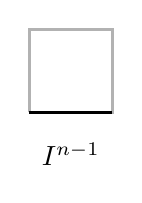
\begin{tikzpicture}[x=3em, y=3em, baseline=1em]
        \draw[very thick, black!30] (0,0)--(1,0)--(1,1)--(0,1)--(0,0);
        \draw[very thick]
        (0,0)--(1,0);
        \filldraw (0.5, -0.5) node{$I^{n-1}$};
    \end{tikzpicture}
    \ar[r, hook]
    &
    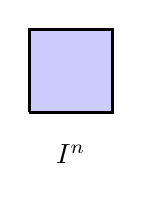
\begin{tikzpicture}[x=3em, y=3em, baseline=1em]
        \filldraw[very thick, fill=blue!20] (0,0)--(1,0)--(1,1)--(0,1)--(0,0);
        \filldraw (0.5, -0.5) node{$I^{n}$};
    \end{tikzpicture}
    & 
    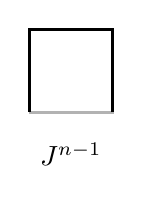
\begin{tikzpicture}[x=3em, y=3em, baseline=1em]
        \draw[very thick, black!30] (0,0)--(1,0)--(1,1)--(0,1)--(0,0);
        \draw[very thick] (1,0)--(1,1)--(0,1)--(0,0);   \filldraw (0.5, -0.5) node{$J^{n-1}$};
    \end{tikzpicture}
    \ar[l, hook]
    \end{tikzcd}
    \)
\end{center}
The \textbf{relative homotopy groups} of the triple $(X,A,x_0)$ are defined as triple homotopy classes of triple maps:
\[\pi_n(X,A,x_0)=[(I^n, I^\ni, J^\ni),(X,A,x_0)].\]
Addition on $\pinr$ for $n\geq 2$ is defined by "juxtaposition and reparametrization in the first coordinate" as follows:
\[[f]+[g]=[f+g],\ (f+g)(\nn{t}{n})=\begin{cases}f(2t_1,\dots,t_n) & t_1\in[0,1/2] \\ g(2t_1-1,\dots,t_n) & t_1\in[1/2,1]\end{cases}\]
this is easily seen to be well defined on homotopy classes.

The \textbf{relative Hurewicz map} is defined similarly to the absolute one: with $c\in H_n(I^n,\de I^n;\Z)$ a generator, define
\[h:\pi_n(X,A,x_0)\to H_n(X,A;\Z),\ [f]\mapsto f_*(c)\]


Recall that $\pi_1(A,x_0)=[(I',\de I'),(A,x_0)]$ acts on $\pi_n(X,A,x_0)$ in a non-trivial fashion. This poses a problem, because for all $[f]\in\pi_n(X,A,x_0)$ and $\omega\in\pi_1(S,x_0)$ the maps representing $[\omega]*[f]$ and $[f]$ are pair-homotopic as maps $(I^n,\de I^n)\to(X,A)$, hence the relative Hurewicz map takes them to the same class in $H_n(X,A;\Z)$.

This leads to the definition of a \textbf{modified relative Hurewicz map}. For $n\geq2$ define $\pinr^\dagger$ to be the quotient of $\pinr$ by the normal subgroup generated by elements of the form $([\omega]*[f])[f]^{-1}$ for all $[\omega]\in\pi_1(A,x_0)$, $[f]\in\pinr$. By design the relative Hurewicz map factors through this quotient:
\begin{center}
    \begin{tikzcd}
        \pinr \arrow[r, "h"] \arrow[d] & \hnr \\
        \pinr^\dagger \arrow[ur, dashed, "h^\dagger" below]
    \end{tikzcd}
\end{center}

Now we can state the relative Hurewicz theorem.

\begin{theorem}[Hurewicz]\label{theorem:hurewicz}
Let $(X,A)$ be a pair of path connected spaces such that for all $x_0\in A$, the map $\pi_1(A,x_0)\to\pi_1(X,x_0)$ is an isomorphism. Let $n\geq2$ and suppose that $\pi_i(X,A,x_0)=0$ for $1\leq i\leq n-1$. Then the modified relative Hurewicz map $h^\dagger$ is an isomorphism.
\end{theorem}

\begin{remark}
For $A=\{x_0\}$, the relative version recovers the absolute version.
\end{remark}

\begin{remark}
The hypothesis of the relative Hurewicz theorem refers to $\pi_i(X,A,x_0)$ but the conclusion refers to $\pi_n(X,A,x_0)^\dagger$. This makes the relative version not as manageable as the absolute one.
\end{remark}
%%% Lecture 2

\section{Some Consequences of Hurewicz Theorem}

\lecture[Getting rid of the basepoint.]{2021-10-13}

Before resuming with the proof of the relative Hurewicz theorem we prove an application of it, a version of Whitehead's theorem which uses homology groups in place of homotopy groups.

\begin{theorem}
Let $f:X\to Y$ be a map between simply connected CW-complexes such that $f_*:H_i(X;\Z)\to H_i(Y;\Z)$ is an isomorphism for all $i\geq 0$. Then $f$ is an homotopy equivalence.
\end{theorem}

\begin{proof}
By cellular approximation we can assume $f$ cellular. Let $Z(f)=X\times[0,1]\cup_{X\times1, f}Y$ be the mapping cylinder of $f$. This inherits a CW-structure such that $X\cong X\times0$ and $Y$ are subcomplexes. The projection $Z(f)\to Y$ is a homotopy equivalence (fact check this), hence by replacing $Y$ by $Z(f)$ we can assume wlog that $f:X\to Y$ is the inclusion of a subcomplex. Since $X$ and $Y$ are simply-connected the relative Hurewicz theorem applies for all $n\geq2$, but all relative homology groups vanish because $f_*$ is an isomorphism (by the long exact sequence), hence all relative homotopy groups vanish and by Whitehead's theorem we can conclude that $f$ is an homotopy equivalence.
\end{proof}

An elaboration of the previous results leads to the following proposition.

\begin{proposition}
Let $f:X\to Y$ be a map of path-connected CW-complexes. The following are equivalent:
\begin{itemize}
    \item[(i)] $f$ is a homotopy equivalence,
    \item[(ii)] $f$ induces an isomorphism on fundamental groups and the induced map $\til{f}:\til{X}\to\til{Y}$ on universal covers induces an isomorphism on all integral homology groups.
\end{itemize}
\end{proposition}

\begin{proof}
$(i)\implies(ii)$ Since $f$ is an homotopy equivalence, $f_*$ is an isomorphism on all homotopy groups. Then $\til{f}$ induces an isomorphism on all homotopy groups, hence it is an homotopy equivalence, thus it induces an isomorphism on all homology groups.

$(ii)\implies(i)$ Since $\til{f}$ induces an isomorphism on integral homology groups it is a homotopy equivalence by the version of Whitehead's theorem we just proved, hence it induces an isomorphism on all homotopy groups. This in turn means that $f$ induces an isomorphism on all homotopy groups, i.e. it is a homotopy equivalence.
\end{proof}

\section{Getting Rid of the Basepoint}

We now return to the proof of the relative Hurewicz theorem

Recall: the \textbf{degree} of a map $f:(D^n,\de D^n)\to(D^n,\de D^n)$ is the integer $\deg(f)$ such that $f_*(x)=\deg(f)x$ for all $x\in H_n(D^n,\de D^n;\Z)$.

\begin{lemma}\label{lemma:degree-of-sphere-self-maps}
Let $n\geq1$. For $n>1$ assume known that $\pi_\ni(\sni,z)$ is free abelian of rank $1$. Let $f$ be a continuous self map of $\sph$ of degree $\pm 1$. Then $f$ is pair-homotopic to the identity if $\deg(f)=1$ and to any reflection if $\deg(f)=-1$.
\end{lemma}

\begin{proof}
We first see the case when $\deg(f)=1$.

$(n=1)$ Since $\de D^1=\cb{\pm1}$ and $\deg(f)=1$ we have $f|_{\de D^1}=\id_{\de D^1}$. Then the linear homotopy $H(x,t)=tf(x)+(1-t)x$ is a relative homotopy between $f$ and the identity $id_{D^1}$.

$(n\geq2)$ Consider the commutative square:
\begin{center}
    \begin{tikzcd}
    H_n(\dn,\de\dn;\Z) \arrow[d,"f_*=\id"] \arrow[r, "\de", "\cong" below] & H_\ni(\sni;\Z) \arrow[d, "(f|_{S^\ni})_*=\id"] \\
    H_n(\dn,\de\dn;\Z) \arrow[r, "\de", "\cong" below] & H_\ni(S^\ni;\Z)
    \end{tikzcd}
\end{center}
Since $\pi_\ni(S^\ni,z)$ is free of rank $1$, the Hurewicz map $h:\pi_\ni(S^\ni,z)\to H_\ni(S^\ni;\Z)$ is an isomorphism. Then $(f|_{\de\dn})_*:\pi_\ni(\sni,z)\to\pi_\ni(\sni,z)$ is the identity, therefore $f|_{\de\dn}$ is homotopic to the identity of $\sni$. Now let $H:\sni\times [0,1]\to\sni$ be a homotopy. This gives a map $D^n\times0\cup\sni\times[0,1]\cup \dn\times1\xto{f\cup H\cup\id}\dn$. Since $\dn\times[0,1]$ can be obtained from $D^n\times0\cup\sni\times[0,1]\cup \dn\times1$ by attaching an $(n+1)$-cell and $\dn$ is contractible\normalmarginpar\marginnote{\footnotesize Why do we need $\dn$ contractible? Think of $S^1\hookrightarrow D^2$}, there is a continuous extension $\bar{H}:\dn\times[0,1]\to\dn$. This is the desired pair homotopy from $f$ to $\id_{\dn}$.

If $\deg(f)=-1$, we let $r:\dn\to\dn$ be the reflection in the first coordinate. Then $\deg(r\circ f)=1$, hence $r\circ f$ is pair homotopic to $\id_{\dn}$ and so $f=r\circ r\circ f$ is pair homotopic to $r$.
\end{proof}

Now let $(X,A)$ be a based space. Define the group $\pi_n(X,A)^\#$ as the quotient of the free abelian group generated by pair homotopic maps $(I^n,\de I^n)\to (X,A)$ by the relation $[f]+[f']=[f+f']$ when the right hand side is defined.

The "forgetful" map $\pinr\to\pi_n(X,A)^\#$ is a group homomorphism and it factors through a homomorphism $\pinr^\dagger\to\pi_n(X,A)^\#$ (because $\omega * f$ and $f$ are always pair homotopic).

\begin{proposition}
Let $(X,A)$ be a pair of path-connected spaces. Let $n\geq2$ or $n=1$ and $A$ a point. Then the "forgetful" homomorphism $\pinr^\dagger\to\pi_n(X,A)^\#$ is an isomorphism.
\end{proposition}

\begin{proof}
We will define a homomorphism in the opposite direction. Let $f:(I^n,\de I^n)\to (X,A)$ be a pair map. $f$ need not send $J^\ni$ to $x_0$, but $J^\ni$ is contractible and $A$ path-connected. So $f|_{J^\ni}$ is homotopic in A to the constant map at the basepoint. Let $H:J^\ni\times[0,1]\to A$ be such a homotopy from $f|_{J^\ni}$ to the constant map $x_0$. The HEP for $(\de I^n,J^\ni)$ lets us extend $H$ to a homotopy $H':\de I^n\times[0,1]\to A$ from $f|_{\de I^n}$ to some map $H'(1,-)$ that sends $J^\ni$ to $x_0$. The HEP for $(I^n,\de I^n)$ with target space $X$ lets us extend $H'$ to $H'':I^n\times[0,1]\to X$ from $f$ to a map that sends $J^\ni$ to $x_0$. Moreover $H''$ is a pair homotopy of maps $(I^n,\de I^n)\to (X,A)$.

We now define a map $\Psi:[(I^n,\de I^n)\to (X,A)]\to \pi_n(X,A,x_0)^\dagger$ by sending $[f]$ to $[H''(-,1)]$. We claim that this is well defined.
 
Claim. Let $f,f':(I^n,\de I^n, J^\ni)\to(X,A,x_0)$ be triple maps that are pair homotopic as maps $(I^n,\de I^n)\to (X,A)$. Then they represent the same element in $\pi_n(X,A,x_0)^\dagger$.
 
\textit{Proof of the claim.} Let $H:I^n\times[0,1]\to X$ be a pair homotopy from $f$ to $f'$. We choose a point $z\in J^\ni$ and a triple homotopy $K:\triple\times[0,1]\to\triple$ from the identity to a map with $K(J^\ni\times 1)=\{z\}$. Formally what we are applying two times the HEP (for $(\de I^n,J^\ni)$ and for $(I^n,\de I^n)$, as before). Then $f$ is triple homotopic to $f\circ K(-,1)$, $f'$ is triple homotopic to $f'\circ K(-,1)$, so that $f\circ K(-,1)$ is pair homotopic to $f'\circ K(-,1)$. In particular $\til{H}=H \circ K(-,1)$ satisfies $\til{H}(J^\ni,t)=H(z,t)$ for all $t\in [0,1]$. Now for all $x\in J^\ni$, the loop at $x_0$ in $A$, $\til{H}(x,-)$, is independent of the point $x\in J^\ni$ and it always agrees with $\omega=\til{H}(z,-)$. By identifying $I^{n+1}$ as $I^n\times[0,1]$ we can view $\til{H}$ as a triple homotopy between $\omega * (f\circ K(-,1))$ and $f'\circ K(-,1)$.\normalmarginpar\todo{I'm not \textit{too} sure I really get this...} In the end we have $[f]=[\omega * (f\circ K(-,1))]=[f'\circ K(-,1)]=[f']$ in $\pinr^\dagger$ (the second equality holds in $\pinr^\dagger$ by construction, the third one is because of the homotopy we found).

\textit{Corollary of the claim.} The map $\Psi:[(I^n,\de I^n),(X,A)]\to\pinr^\dagger$ we defined before the claim is well defined, so it has a unique extension on the free abelian group which factors to a homomorphism $\pi_n(X,A)^\#\to\pinr^\dagger$ which is then an isomorphism by design.
\end{proof}
 
Punchline: In the situation of the relative Hurewicz theorem it suffices to show that the map $\pi_n(X,A)^\#\to H_n(X,A;\Z)$ is an isomorphism (i.e. we don't have to deal with basepoints!).

%%% Lecture 3

\section{The Homotopy Addition Theorem}

\lecture[The Homotopy Addition Theorem: a theorem which is necessary, but a pain to prove.\newline---\emph{\enquote{When homotopy theory was new, people thought this was obvious and didn't feel the need for a proof, until Eilenberg suggested so.}}]{2021-10-18}

This lecture was given by Tobias Lenz, a PhD student of Schwede. I was late to the class, so most of the notes for this lecture are copied from Qi Zhu's notes, thank you Qi Zhu!

\begin{remark}
There's a standing assumption for all of today's lecture: $\pi_k(S^k)\cong\Z$ for all $1\leq k<n$.
\end{remark}

The main goal of today's lesson is to prove the following theorem.

\begin{theorem}[Homotopy Addition Theorem]\label{theorem:HAT}
Assume we have $\nn{f}{k}:I^n\to I^n$ such that $f_i|_{\ring I^n}$ is an open embedding and the sets $f_i(\ring I^n)$ are pairwise disjoint. Furthermore, let $g:\pair\to (X,A)$ such that $g(I^n\sm\bigcup_{i=1}^k f_i(\ring I^n))\subset A$. Then
\[[g]=\sum_{i=1}^k(\deg f_i)[g\circ f_i]\]
in $\pi_n(X,A)\#$.
\end{theorem}

\begin{remark}
Note that we have $f_i(\de I^n)\cap f_j(\ring I^n)=\emptyset$ for all $i,j$. This will play a (small) role later in the lecture.
\end{remark}

\begin{remark}
Two remarks about the theorem:
\begin{itemize}
    \item When homotopy theory was new, people thought this was obvious and didn't feel the need for a proof until Eilenberg suggested so.
    \item Tobias: \emph{\enquote{I'm not sure if I can finish the proof today but I was promised an award if I do!}}
\end{itemize}
\end{remark}

\begin{center}
\begin{tikzpicture}[x=1.5em, y=1.5em]
\filldraw[very thick, black, fill=blue!20]
    (0,0)--(0,10)--(10,10)--(10,0)--(0,0);
\draw[very thick]
    (-4,4)--(-4,6)--(-2,6)--(-2,4)--(-4,4)
    (-4,1)--(-4,3)--(-2,3)--(-2,1)--(-4,1)
    (-4,7)--(-4,9)--(-2,9)--(-2,7)--(-4,7);
\filldraw[fill=white, use Hobby shortcut,closed=true] 
    (1,5) .. (4,9) .. (7,5) .. (4,8) .. (3,4) .. (5,2) .. (7,5) .. (8,2) .. (5,1);
\filldraw[fill=white, use Hobby shortcut,closed=true] 
    (3,5) .. (3,6) .. (5.3,6) .. (5.4,4);
\path[draw]
    (3,5) -- (3.5,5) -- (3.6,5.5) -- (3.8, 5.5);
\filldraw[fill=white, use Hobby shortcut,closed=true] 
    (8,1) .. (8,2) .. (9.5,2) .. (9.5,1);
\path[draw, -{\tip}, use Hobby shortcut,closed=false]
    (9,7) .. (9.5,7.5) .. (11,8);
\draw 
    (7,6) node {\scriptsize$f_1(I^n)$}
    (8.7,1.5) node {\scriptsize$f_2(I^n)$}
    (4.7,4.9) node {\scriptsize$f_3(I^n)$}
    (11,8) node[anchor=west] {$A$}
    (10,5) node[anchor=west] {$\xrightarrow{\quad g\quad} X$}
    (-2,2) node[anchor=west] {$\xrightarrow{\ f_1\ }$}
    (-2,5) node[anchor=west] {$\xrightarrow{\ f_2\ }$}
    (-2,8) node[anchor=west] {$\xrightarrow{\ f_3\ }$};
\end{tikzpicture}
\end{center}\label{fig:HAT1}\medskip

The strategy to prove this theorem is inductive: we want to reduce the problem to the case $k=1$ which is easy.

\begin{definition}
Let $f:\ring I^n\to\ring I^n $ be an open embedding, $p\in\ring I^n$. We have that $f$ induces a commutative diagram:
\begin{center}
    \begin{tikzcd}
    H_n(\ring I^n,\ring I^n\sm\cb{p}) \arrow[r, "i_*"] \arrow[d, "f_*" left] \arrow[dr, "f_*"] & H_n(I^n,I^n\sm\cb{p}) & H_n\pair \arrow[l, "i_*" above] \arrow[d, red, dashed, "d\cdot-"] \\
    H_n(f(\ring I^n), f(\ring I^n)\sm\cb{f(p)}) \arrow[r, "i_*" below] & H_n(f(I^n),f(I^n)\sm\cb{f(p)}) & H_n\pair \arrow[l, "i_*" below]
    \end{tikzcd}
\end{center}
\end{definition}
where the maps are all isomorphisms by homotopies and excision, hence they induce the dashed arrow. This is an automorphism of $H_n\pair\cong\Z$ and thus $d=\pm1$. One can show this is independent of $p$, hence we call it the \tbf{local degree} of $f$, and write $\deg(f)=d$.

\begin{lemma}
For $1\leq i\leq k$, let $\Uu_i\subset f_i(\ring I^n)$ be any non-empty open set. Then $g$ is homotopic relative to $I^n\sm f_i(\mathring{I}^n)$ to a map that sends $f_i(I^n)\sm\mathcal{U}_i$ to $A$ for all $i$.
\end{lemma}

\begin{remark}
If $[g]=[g']$ in $\pi_n(X,A)^\#$ then $[g\circ f_j]=[g'\circ f_j]$ for all $1\leq j\leq k$.
\end{remark}

\begin{proof}
There is a homotopy relative $\de I^n$ from the identity to a map that sends everything outside of $\ring Q$ to $\de I^n$, where $Q$ is a cube inside $f^{-1}_i(\mathcal{U}_i)$ (basically we take a cube $Q$ inside $f^{-1}_i(\mathcal{U}_i)$ and we blow it to the big cube $\de I^n$ containing $f^{-1}_i(\mathcal{U}_i)$). Composing with $gf_i$ yields a homotopy $H$ of maps of pairs $(I^n,\de I^n)\to(X,A)$ from $gf_i$ to a map that sends everything outside $\ring Q$ to $A$. We have a map of sets:
\[H':I^n\times I\to X,\quad H'(x,t)=\begin{cases}H(f^{-1}(x),t) & x\in f_i(I^n) \\ g(x) & x\not\in f_i(\mathring{I}^n)\end{cases}\]
which we can show is well defined. Let $x\in f_i(\de I^n)$, with preimage $y$, then\normalmarginpar\marginnote{\footnotesize It suffices to check this because $f_i(\de I^n)\cap f_j(\ring I^n)$ is empty for all $i,j$.} \[g(x)=H(y,t)=H(y,0)=gf_i(y)\] so that it is well defined as a map of sets. Then $H'(x,0)=g(x)$ and $H'(x,1)\in A$ for $x\not\in f(\mathring{Q})$, in particular $H'(x,1)\in A$ for $x\not\in\mathcal{U}_i$. It remains to prove that $H'$ is continuous.

Claim. We have a commutative square
\begin{center}
    \begin{tikzcd}[column sep=20mm]
    \de I^n\times I \arrow[d, "i"] \arrow[r, "f_i|_{\de I^n}\times\id"] & (I^n\sm f_i(\ring I^n))\times I \arrow[d, "i"] \\
    I^n\times I \arrow[r, "f_i\times\id"] & I^n\times I
    \end{tikzcd}
\end{center}
Then,
\[(I^n\times I)\amalg_{\de I^n\times I} ((I^n\sm f_i(\mathring{I}^n))\times I)\xto{(f_i\times\id,i)} I^n\times I\]
is a homeomorphism.

\begin{claimproof}
Well-definedness and continuity of the function follow from the universal property of the pushout. One can check that it is bijective by a direct computation. Hence we have a continuous bijection from a quasi-compact space to an Hausdorff space, which is then a homeomorphism. 
\end{claimproof}

Thus to show that $H'$ is continuous, it suffices to show that the maps $H'\circ (f_i\times I)$ and $H'|_{(I^n\sm f(\ring I^n))\times I}$ are continuous, which follows from the construction.\todo{Not sure how this works, to be honest}
\end{proof}

\begin{proof}[Proof of the homotopy addition theorem (\ref{theorem:HAT})]\renewcommand{\qedsymbol}{\textit{To be continued...}} Induction on $k$.

$(k=1)$ Take a cube $Z_1\subset f_1(\mathring{I}^n)$. By the lemma we may assume that $g(I^n\sm\mathring{Z}_1)\subset A$. Our goal is to construct some $f_1':(I^n,\de I^n)\to(I^n,\de I^n)$ with $[gf_1]=[gf_1']$. There exists\normalmarginpar\marginnote{\footnotesize The homotopy $Q$ is the same kind of "pushing out" homotopy that we already considered in the proof of the lemma.} a homotopy $Q$ from $\id_{I^n}$ to a map $p$ such that:
\begin{itemize}
    \item $p|_{Z}=\id_{Z}$, where $Z$ is a cube inside $Z_1$,
    \item $p(I^n\sm\mathring{Z}_1)\subset\de I^n$,
    \item $Q((I^n\sm\mathring{Z}_1)\times I)\subset I^n\sm \mathring{Z}_1$.
\end{itemize}
Now, $Qf_1$ is a homotopy of maps of pairs $(I^n,\de I^n)\to(I^n,I^n\sm\mathring{Z}_1)$. Then $gQf_1$ will be a homotopy of maps of pairs $(I^n,\de I^n)\to(X,A)$, hence $[gpf_1]=[gf_1]$ in $\pi_n(X,A)^\#$. Then $f_1':= pf_1$ is a map of pairs $(I^n,\de I^n)\to(I^n,\de I^n)$ and $f_1\simeq f_1'$ as maps of pairs $(I^n,\de I^n)\to(I^n,I^n\sm \mathring{Z}_1)$.

Claim.\reversemarginpar\marginnote{\footnotesize We are dealing with two different notions of degree, the usual one for $f'_1$ and the local degree for $f_1$.} $\deg f_1$ equals the degree of $f_1'$ as a map $(I^n,\de I^n)\to(I^n,\de I^n)$.

\begin{claimproof}
Consider the diagram:
\begin{center}
    \begin{tikzcd}[column sep=small]
    H_n(\mathring{I}^n,\mathring{I}^n\sm\cb{x}) \arrow[r, "i_*",] \arrow[d, "(f_1)_*" left] & H_n(I^n,I^n\sm\cb{x}) \arrow[d, "(f_1)_*"] & H_n(I^n,\de I^n) \arrow[l, "i_*" above] \arrow[d, shift left, "(f_1)_*\ \," left] \arrow[d, shift right, "\ \,(f'_1)_*" right] \arrow[dr, "(f'_1)_*"] \\
    H_n(\mathring{I}^n, \mathring{I}^n\sm\cb{f_1(x)}) \arrow[r, "i_*"] & H_n(I^n,I^n\sm\cb{f_1(x)}) & H_n(I^n,I^n\sm \mathring{Z}_1) \arrow[l, "i_*" above] & H_n\pair \arrow[l, "i_*"]
    \end{tikzcd}
\end{center}
we have that the parallel arrows agree, which proves the claim.
\end{claimproof}

Now, if $\deg f_1=1$, then $f_1'\simeq\id$ as maps of pairs, hence $(\deg f_1)[gf_1]=[gf_1']=[g]$.

If instead $\deg f_1=-1$, then $f_1'\sim r$ where $r$ is reflection in the first coordinate by lemma \ref{lemma:degree-of-sphere-self-maps}, hence $[g]=-[gr]=-[gf_1']=-[gf_1]=(\deg f_1)[gf_1]$.

\end{proof}

%%% Lecture 4

\lecture[We finish the proof of the HAT. My first non-trivial homotopy groups.]{2021-10-25}
$(k\geq2)$ Set $u_i=f_i(\text{center of } I^n)\in I^n$. Assume without loss of generality that the first coordinates of $\nn{u}{k}$ are not all equal (if some of them are, we can "wiggle" $f_1$).

\begin{center}
\begin{tikzpicture}[x=0.7em, y=0.7em, baseline=0.7*5em]
\filldraw[very thick, black, fill=blue!20]
    (0,0)--(0,10)--(10,10)--(10,0)--(0,0);
\filldraw[fill=white, use Hobby shortcut,closed=true] 
    (1,5) .. (4,9) .. (7,5) .. (4,8) .. (3,4) .. (5,2) .. (7,5) .. (8,2) .. (5,1);
\filldraw[fill=white, use Hobby shortcut,closed=true] 
    (4,5) .. (4,6) .. (5.3,6) .. (5.4,4);
\filldraw[fill=white, use Hobby shortcut,closed=true] 
    (8,1) .. (8,2) .. (9,2) .. (9,1);
\draw 
    (7,6) node {\scriptsize$f_1$}
    (8.5,1.5) node {\scriptsize$f_2$}
    (5.2,4.9) node {\scriptsize$f_3$};
\end{tikzpicture}
$\xrightarrow{\text{shrink domains to}}$
\begin{tikzpicture}[x=0.7em, y=0.7em, baseline=0.7*5em]
\filldraw[very thick, black, fill=blue!20]
    (0,0)--(0,10)--(10,10)--(10,0)--(0,0);
\filldraw[fill=white, use Hobby shortcut,closed=true] 
    (1,5) .. (2,6) .. (3,5) .. (2.5,3);
\filldraw[fill=white, use Hobby shortcut,closed=true] 
    (4,5) .. (4,6) .. (5.3,6) .. (5.4,4);
\filldraw[fill=white, use Hobby shortcut,closed=true] 
    (8,1) .. (8,2) .. (9,2) .. (9,1);
\draw[dashed] (3.5,0)--(3.5,10) (6.5,0)--(6.5,10);
\draw 
    (2,5) node {\scriptsize$f_1$}
    (8.5,1.5) node {\scriptsize$f_2$}
    (5.2,4.9) node {\scriptsize$f_3$};
\end{tikzpicture}
$\xrightarrow{\text{blow images to}}$
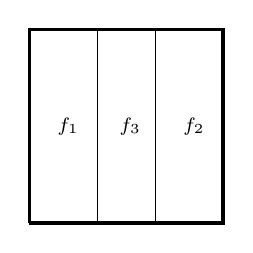
\begin{tikzpicture}[x=0.7em, y=0.7em, baseline=0.7*5em]
\draw[very thick, black]
    (0,0)--(0,10)--(10,10)--(10,0)--(0,0);
\draw (3.5,0)--(3.5,10) (6.5,0)--(6.5,10);
\draw 
    (2,5) node {\scriptsize$f_1$}
    (8.5,5) node {\scriptsize$f_2$}
    (5.2,5) node {\scriptsize$f_3$};
\end{tikzpicture}
\end{center}

\hspace*{\fill}$\leadsto [g] = \sum[g\circ f_i].$


Choose $t\in (0,1)$ such that
\begin{itemize}
    \item $t$ is different from the first coordinates of $\nn{u}{k}$,
    \item for some $1\leq i\leq k$, the first coordinate of $u_i$ is smaller than $t$,
    \item for some $1\leq i\leq k$, the first coordinate of $u_i$ is larger than $t$.
\end{itemize}

Choose neighborhoods $\Uu_i$ of $u_i$ inside $f_i(\ring I^n)$ that do not intersect $\cb{t}\times I^\ni$, that is such that $\Uu_i$ lies "on the same side respect to $t$" as $u_i$.

Choose subcubes $Q_i$ inside $\ring I^n$ that contain the center and lie in in $f^{-1}(\Uu_i)$.

Last time we proved that $g$ is pair-homotopic to some $g':\pair\to\pairs$ such that
\[g'(I^n\sm\bigcup_{i=1,\dots,k} f_i(Q_i))\subset A\quad\text{and}\quad[g\circ f_i]=[g'\circ f_i]\text{ in }\pi_n\pairs^\#.\]

We precompose each $f_i:I^n\to I^n$ with the linear shrinking homotopy relative $Q_i$. Set $f'_i=f_i\circ \text{ end of shrinking}$. Then $g'\circ f_i$ is pair homotopic to $g'\circ f'_i$ and $f'_i(I^n)\subset\Uu_i$.

By replacing $g$ by $g'$ and $f_i$ by $f'_i$ we can therefore assume without loss of generality that $f_i(\ring I^n)$ lies on one side of $\cb{t}\times I^\ni$.

\begin{center}
\begin{tikzpicture}[x=0.7em, y=0.7em, baseline=0.7*5em]
\filldraw[very thick, black, fill=blue!20]
    (0,0)--(0,10)--(10,10)--(10,0)--(0,0);
\filldraw[fill=white, use Hobby shortcut,closed=true] 
    (1,5) .. (2,6) .. (3,5) .. (2.5,3);
\filldraw[fill=white, use Hobby shortcut,closed=true] 
    (4,5) .. (4,6) .. (5.3,6) .. (5.4,4);
\filldraw[fill=white, use Hobby shortcut,closed=true] 
    (8,1) .. (8,2) .. (9,2) .. (9,1);
\draw[dashed] (3.5,0)--(3.5,10);
\draw 
    (2,5) node {\scriptsize$f_1$}
    (8.5,1.5) node {\scriptsize$f_2$}
    (5.2,4.9) node {\scriptsize$f_3$};
\end{tikzpicture}
\end{center}\smallskip

Write $g=g_1+_t g_2$ by "cutting along $\cb{x_1=t}$".

Formally, $g_1(\xs)=g(t\xs)$ and $g_2=g((1-t)x_1+t,\dots,x_n)$.

Set $I_1=\cb{i\in I\mid u_i\text{ lies left of }\cb{x_1=t}}$ and $I_2=\cb{i\in I\mid u_i\text{ lies right of }\cb{x_1=t}}$, where $I=\cb{1,\dots,k}$.

Then by the inductive hypothesis:
\[[g]=[g_1]+[g_2]=\sum_{i\in I_1}\deg(f_i)[g_1\circ f_i]+\sum_{i\in I_2}\deg(f_i)[g_2\circ f_i]=\sum_{i\in I}\deg(f_i)[g\circ f_i].\]\qed

\begin{remark}
Note that we have proved the HAT \textit{assuming} (in order to use lemma \ref{lemma:degree-of-sphere-self-maps}) that $\pi_{n-1}(S^{n-1},*)\cong\Z$, not in full generality! This is enough to prove \ref{theorem:my-first-non-trivial-homotopy-group} which in turn will prove the HAT in each dimension. This is essentially an (awfully confusing) inductive argument!
\end{remark}

\section{My First Non-Trivial Homotopy Group}

\begin{theorem}\label{theorem:my-first-non-trivial-homotopy-group}
Let $n\geq2$ and assume inductively that $\pi_{n-1}(S^{n-1},*)\cong\Z$ so that the HAT holds in dimension $n$. Then $\pi_n(S^n,*)$ is infinite cyclic.
\end{theorem}

\begin{proof}
Choose some point $z\in S^n$. Set $U=S^n\sm\cb{-z}$. Then \[\pi_n(S^n,z)=\pi_n(S^n,\cb{z},z)\underset{U\cong *}{\cong}\pi_n(S^n,U,z)\underset{\pi_1(U,z)=\cb{1}}{\cong}\pi_n(S^n,U,z)^\dagger\cong\pi_n(S^n,U)^\#\]
So we may show that $\pi_n(S^n,U)^\#\cong\Z$.

We show that $\pi_n(S^n,U)^\#$ is generated by the class of any pair map $\psi:\pair\to(S^n,U)$ such that $\psi(\de I^n)=\cb{z}$ and $\psi$ factors out a homeomorphism $I^n/\de I^n\cong S^n$.

Let $f:(I^n,\de I^n)\to(S^n,U)$ be any pair map. Set $V=S^n\sm\cb{z}$ so that $S^n=U\cup V$ is an open cover.

The Lebesgue Number lemma provides an $m\geq1$ so that each subcube of $I^n$ of side length $1/m$ is mapped by $f$ into $U$ or into $V$. Decompose $I^n$ into $m^n$ subcubes of side length $1/m$.

We define subspaces of $I^n$ in this way:
\begin{itemize}[label=-]
    \item $A_{-1}=\de I^n$
    \item $A_0=A_{-1}\cup\cb{\text{\,vertices of the }m^n\text{ subcubes}}$
    \item $A_1=A_0\cup\cb{\text{\,edges of the }m^n\text{ subcubes}}$
    \item $A_2=\cdots$
    \item $A_n=I^n$
\end{itemize}

We want to "improve" $f$ successively by pair homotopies to maps $f=f_{-1},f_0,f_1,\dots,f_{n-1}$ such that:
\begin{itemize}
    \item each $f_j$ is homotopic to $f$ relative $\de I^n$,
    \item each $f_j$ is admissible, i.e. it sends every subcube of side length $1/m$ to $U$ or to $V$,
    \item $f_j(A_j)\subset U$ for $j=-1,0,1,\dots,n-1$.
\end{itemize}

We proceed by induction on $j$. There is nothing to show for $j=-1$. Let now $j\geq 0$. We first modify $f_{j-1}$ and the faces of the $j$-cube. If such a face $Q$ is "good", i.e. sent by $f_{j-1}$ into $U$, we do not do anything to $Q$. Otherwise the $(j-1)$-subcube is mapped to $V$ and the restriction of $f_{j-1}$ to it is a pair map $(Q,\de Q)\to (V,V\cap U)$.

Claim. For $j<n$, any pair map $(I^j,\de I^j)\to (V,U\cap V)$ is homotopic relative $\de I^j$ to a map with image in $U\cap V$.

\begin{claimproof}
By stereographic projection $(V,U\cap V)$ is pair homotopic to $(\R^n,\R^n\sm\cb{0})$, i.e. we can construct a pair map $g:(I^j,\de I^j)\to (\R^n,\R^n\sm\cb{0})$. Because $\de I^j$ is compact and $0\notin f(\de I^j)$, there is an $\epsilon>0$ such that $g(\de I^j)\cap(\epsilon\text{-ball around }0)=\emptyset$.

So $g:(I^j,\de I^j)\to(\R^n,\R^n\sm\ring B(\epsilon,0))$. Now, $\R^n$ can be obtained from $\R^n\sm\ring B(\epsilon,0)$ by attaching an $n$-cell. The cellular approximation theorem and the fact that $I^j$ is a $j$-dimensional CW-complex gives us a relative homotopy from $g$ to a cellular map. Since $j<n$, the cellular map has image in $\R^n\sm\ring B(\epsilon,0)\subset\R^n\sm\cb{0}$.
\end{claimproof}

We can now change $f_{j-1}|A_j$ into $f_j|A_j$ by a homotopy relative $A_{j-1}$ into a map that sends all $j$-cells to $U$.

We use the HEP for $(I^n,A_j)$ to extend $f_j$ to all of $I^n$; we use the HEP with target $U$ or with target $V$ to ensure that the map $f_j$ is again admissible.

After this inductive construction we can replace $f$ by $f_{n-1}$ and we have arranged without loss of generality that $f(A_{n-1})\subset U$.

We can now assume that $g:\pair\to(S^n,U)$ satisfies $g(A_{n-1})\subset U$ and each top-dimensional subcube is mapped to $U$ or to $V$.

We apply the HAT to this map $g$ with $\nn{f}{k}$ the reparametrization of those subcubes that are \textit{not} mapped into $U$ (and hence into $V$).

Then by the HAT we have:
\[[g]=\sum_i\pm[g\circ f_i]\text{ in }\pi_n(S^n,U)^\#\cong\pi_n(S^n,\cb{z},z)^\dagger\cong\pi_n(S,z)\]

We have gained that each summand on the right hand side is in the image of the homomorphism $\pi_n(V,V\cap U)^\#\to\pi_n(S^n,U)^\#$, which is then surjective. By the long exact homotopy group sequence of the pair $(V,V\cap U)$, we obtain:
\[\pi_n(V,V\cap U,z)=\pi_n(\R^n,\R^n\sm\cb{0},z)\cong\pi_\ni(\R^{n-1}\sm\cb{0},z)\cong\pi_\ni(S^\ni,z)\cong\Z\]
so $\pi_n(S^n,U)^\#$ is infinite cyclic.
\end{proof}

\section{Reminder on Simplicial Sets}\label{section:reminder-on-sset}
\todo{Maybe I will add something more about the basics of simplicial sets in the appendix.}
We denote by $\Delta$ the category with objects the sets $[n]=\cb{0,1,\dots,n}$, $n\geq 0$ and morphisms the weakly monotone maps.

A \textbf{simplicial set} is a contravariant functor from $\Delta$ to sets, $X:\Delta^\op \to\Set$. The set of the $n$-simplices is denoted $X_n=X([n])$, for a morphism $\alpha:[n]\to[m]$ write $\alpha^*=X(\alpha):X_m\to X_n$.

The \textbf{singular complex} (singular simplicial set) of a space $Y$ is the simplicial set
\[\S(Y):\Delta^\op \to\Set, \quad [n] \mapsto \S(Y)_n :=\left\{\text{continuous maps }f:\nabla^n \to Y\right\},\]
where $\nabla^n=\{(\xso)\in\R^{n+1}\mid x_i\geq0,\ \sum x_i=1\}$.

For $\alpha: [n]\to [m]$, the map $\alpha^*:\S(Y)_m\to\S(Y)_n$ is precomposition with the affine linear map $\alpha_*:\nabla^n\to\nabla^m$ defined by $e_i\mapsto e_{\alpha(i)}$ (i.e. the map $(\nno{t}{m})\mapsto\alpha_*(t)_j=\sum_{j=\alpha(i)}t_j$).

For a continuous map $\psi:Y\to Z$, a morphism of simplicial sets $\psi_*:=\S(\psi):\S(Y)\to\S(Z)$ is given by $\S(\psi)_n(f)=\psi\circ f$. This yields a functor $\S:\Top\to\sSet$.

The \textbf{geometric realization} is a functor $|-|:\sSet\to\Top$ defined as follows. For a simplicial set $X$ we set
\[|X|=\left(\coprod X_n\times\nabla^n\right)/\sim\]
where $X_n$ is endowed with the discrete topology and the equivalence relation is the one generated by:\normalmarginpar\marginnote{\footnotesize The equivalence relation is only \textit{generated} by the condition stated, which is not symmetric. The actual equivalence relation is not easy to understand. We will return on this problem with the theory of minimal representatives in chapter \ref{subsection:minimal-representatives}.}
\[X_m\times\nabla^m\cont(x,\alpha_*(t))\sim(\alpha^*(x),t)\in X_n\times\nabla^n\quad\text{for all }\alpha:[n]\to[m],\ x\in X_m,\ t\in\nabla^n.\]

\reversemarginpar

%%% Lecture 5

\lecture[A lot of simplicial stuff.]{2021-10-27}

Given two simplicial sets $X$ and $Y$, their product $X\times Y$ is the functor \[\Delta^\op\xto{(X,Y)}\Set\times\Set\xto{\times}\Set\] i.e. $(X\times Y)_n=X_n\times Y_n$ and $\alpha^*_{X\times Y}=\alpha^*_X\times\alpha^*_Y$.

The \textbf{simplicial $n$-simplex} is the represented simplicial set $\Delta[n]:=\Delta(-,[n])$. By the Yoneda lemma, for every simplicial set $X$, the map $\sSet(\Delta[n],X)\to X_n$, $(f:\Delta[n]\to X)\mapsto f_n(\id_{[n]})$.

A \textbf{homotopy between morphisms} $f,g:X\to Y$ in $\sSet$ is a morphism $H:X\times\Delta[1]\to Y$ such that $H\circ i_0=f$ and $H\circ i_1=g$, where $i_0,i_1:X\to X\times\Delta[1]$ (note: the morphism $i_0$ has components $(i_0)_n:X_n\to X_n\times\Delta([n],[1])$, $x\mapsto(x,\text{cost}_0)$).

The topological simplex $\nabla^n=\cb{(\xso)\in\R^{n+1}\mid x_i\geq0,\ \sum x_i=1}$ has a preferred CW-structure with $\sk_k(\nabla^n)=\cb{(\xso)\in\nabla^n\mid\text{at most }k+1\text{ cordinates are non-zero}}$, i.e. $\sk_k(\ns)$ is the union of all $k$-dimensional faces of $\ns$:
\begin{itemize}
    \item $\sk_0(\nabla^n)=\cb{\nno{e}{n}}$,
    \item $\sk_j=\dots$
    \item $sk_{n-1}(\nabla^n)=\de\nabla^n$,
    \item $\sk_n(\nabla^n)=\nabla^n$.
\end{itemize}\medskip

Let $(X,A)$ be a space pair and $k\geq-1$. We define a \textbf{simplicial subset} $\S(X,A,k)$ of $\S(X)$ by
\[S(X,A,k)_n=\cb{f:\ns\to X\mid f(\sk_k(\ns))\subset A}\]
this is indeed a simplicial subset because the affine linear maps $\alpha_*:\ns\to\ms$ are cellular.

Note that we have:

\[\S(X)=\S(X,A,-1)\supset \S(X,A,0)\supset \S(X,A,1)\supset\dots\supset\bigcap_{k\geq1}\S(X,A,k)=\S(A)\]

A space pair $(X,A)$ is \textbf{$k$-connected}, $h\geq0$, if the following equivalent conditions hold:
\begin{enumerate}[label={(\alph*)},topsep=0.5\thmsep]
    \item The inclusion $A\hto X$ is a bijection on $\pi_i$ for all $i<k$ and all basepoints in $A$ and a surjection on $\pi_k$,
    \item Every pair map $(D^n,\de D^n)\to (X,A)$ for $0\leq n\leq k$ is homotopic relative $\de D^n$ to a map with image in $A$,
    \item The map $\pi_0(A)\to \pi_0(X)$ is surjective and $\pi_i(X,A,x)=\cb{*}$ for all $1\leq i\leq k$ and all $x\in A$.
\end{enumerate}

We want to prove the following theorem.

\begin{theorem**}
Let $(X,A)$ be a $k$-connected pair of spaces. The inclusion $\S(X,A,k)\hto\S(X)$ is then a deformation retraction of simplicial sets.
\end{theorem**}

This means there is a simplicial homotopy
\[H:S(X)\times\Delta[1]\to S(X)\]
from the identity to a morphism with image in $\S(X,A,k)$ that is relative to $\S(X,A,k)$, i.e. the restriction of $H$ to $S(X,A,k)$ is the composite
\[\S(X,A,k)\times\Delta[1]\xto{\text{proj}}\S(X,A,k)\xhto{\text{incl}}\S(X).\]

We first prove a proposition.

Let $X$ be a simplicial set and $x\in X_n$, for $n\geq0$. Then the $n$-simplex $x$ is \textbf{degenerate} if there is a surjective morphism $\sigma:[n]\to [k]$ with $k<n$, and $y\in X_k$ such that $X=\sigma^*(y)$ (i.e. $x\in\im(\sigma^*:X_k\to X_n)$).

\begin{proposition}
Let $X$ be a simplicial set and $x\in X_n$. Then there is a unique pair $(\sigma,y)$ consisting of:
\begin{itemize}
    \item a surjective morphism $\sigma: [n]\to [k]$ and
    \item a non-degenerate simplex $y\in X_k$
\end{itemize}
such that $X=\sigma^*(y)$.
\end{proposition}

\begin{proof}\ 

Existence. By induction on $n$. If $n=0$ then $X$ is non-degenerate and $(\id_{[0]},x)$ does the job.

For $n\geq1$: if $x$ is non-degenerate, then $(\id_{[n]},x)$ does the job.
Otherwise $x=\sigma^*(x')$ for some $\sigma:[n]\to [k]$, $k<n$, $x'\in X_k$.
Then $x'=(\sigma')^*(y)$ for some surjective morphism $\sigma':[k]\to[l]$ and $y\in X_l$ non-degenerate, by induction. Then \[x=\sigma^*(x')=\sigma^*((\sigma')^*(y))=(\sigma'\circ\sigma)^*(y)\] which is the desired expression.

Uniqueness. Let $x=\sigma^*(y)=\bar{\sigma}^*(\bar y)$ for surjective morphisms $\sigma:[n]\onto[k]$, $\bar{\sigma}:[n]\onto[l]$ and $y\in X_k$, $\bar y \in X_l$ non-degenerate.

Let $\delta:[k]\to[n]$ be a morphism in $\Delta$ such that $\sigma\circ\delta=\id_{[k]}$.
Then
\[y=(\sigma\delta)^*(y)=\delta^*(\sigma^*(y))=\delta^*(\bar{\sigma}^*(\bar{y}))=(\bar{\sigma}\delta)^*(\bar{y})\]
We write
\[\bar{\sigma}\delta=\delta'\sigma': [k]\to[l]\]
where $\sigma':[k]\onto[a]$ is surjective and $\delta':[a]\hto[l]$ is injective. Then \[y=(\bar\sigma\delta)(\bar y)=(\delta'\sigma')^*(\bar y)=(\sigma')^*((\delta')^*(\bar{y}))\tag{$*$}\]

Since $y$ is non-degenerate, we must have $a=k$ and $\sigma'=\id_{[k]}$. Hence $k=a\leq l$. By interchanging the roles of $(\sigma,y)$ and $(\bar{\sigma},\bar{y})$ we obtain $l\leq k$, hence $l=k$.

Then by $(*)$ we have $y=(\delta')^*(\bar{y})$ so $\delta'=\id$ and hence $y=\bar{y}$ and $\sigma=\bar{\sigma}$.
\end{proof}

\begin{theorem}\label{sx-def-r}
Let $(X,A)$ be $k$-connected. Then $S(X,A,k)\hookrightarrow S(X)$ is a simplicial deformation retraction.
\end{theorem}

\begin{proof}
We will construct the following data. Continuous maps $\psi_f:\nabla^n\times\nabla^1\to X$ for all $f:\nabla^n\to X$, $n\geq 0$ such that:
\begin{enumerate}[label={(\alph*)}]
    \item $\psi_f(-,e_0)=f$, $\psi_f(\sk_k(\ns),e_1)\subset A$.
    \item If $f(\sk_k(\ns))\subset A$, then $\psi_f=f\circ\pr_1$.
    \item The maps $\psi_f$ are compatible in the simplicial direction, i.e. for all $\alpha:[n]\to[m]$, $g:\nabla^m\to X$, the following commutes:
    \begin{center}
        \begin{tikzcd}
            \nabla^n\times\nabla^1 \arrow[d, swap, "\alpha_*\times\id"] \arrow[r, "\psi_{\alpha^*(g)}"] & X \\
            \nabla^m\times\nabla^1 \arrow[ur, swap, "\psi g"]
        \end{tikzcd}
    \end{center}
\end{enumerate}

Construction of the $\psi_f$'s. By induction on $n\geq0$.

$(n=0)$ The map $f:\nabla^0\to X$ is determined by its image $f(e_0)\in X$. Since $\pi_0(A)\to\pi_0(X)$ is surjective, we can choose a path from $f(e_0)$ to some point in $A$. We view the path as a continuous map $\psi_f:\nabla^0\times\nabla^1\to X$ with $\psi_f(e_0,e_0)=f(e_0)$, $\psi_f(e_0,e_1)\in A$. If $f(e_0)\in A$, we take the constant path at $f(e_0)$.

$(n\geq1)$ We distinguish three cases:

Case 1. $f:\nabla^n\to X_n$ is degenerate as a simplex of the simplicial set $\S(X)$. Then $f=\sigma^*(g)$ for a unique pair $(\sigma,g)$ with $\sigma:[n]\onto[k]$, $k<n$ and $g:\nabla^k\to X$ continuous. By (c) we have to define $\psi_f$ as the composite
\[\nabla^n\times\nabla^1\xto{\sigma_*\times\id}\nabla^k\times\nabla^1\xto{\psi_g} X\]

Case 2. $f:\nabla^n\to X$ is non-degenerate and $k<n$. We note that by property $(c)$, the map $\psi_f:\nabla^n\times\nabla^1\to X$ is already fixed on $(\de\nabla^n)\times\nabla^1$; by $(a)$ it is also determined on $\nabla^n\times e_0$.

We extend the data to $\nabla^n\times\nabla^1$ by a choice of continuous retraction:
\[r:\nabla^n\times\nabla^1\to (\nabla^n\times e_0)\cup(\de\nabla^n\times\nabla^1)\]
hence set $\psi_f$ to be the composite of $r$ and $\til f=f\cup\bigcup_{i=0,\dots,n}\psi_{d_i^*(f)}$\normalmarginpar\marginnote{\footnotesize $d_i:[n-1]\to[n]$ is the unique monotone injection with $i\not\in\im(d_i)$).}:
\[\ns\times\sx{1}\xto{r}(\nabla^n\times e_0)\cup(\de\nabla^n\times\nabla^1)\xto{\til f} X\]

The definition satisfies $\psi_f(-,e_0)=f$ by design and $\psi_f(\sk_k(\nabla^n),e_1)\subset\psi_f(\de\nabla^n,e_1)\subset A$ by induction because $\psi_{d_i^*(f)}$ have property $(a)$.

Case 3. $f:\nabla^n\to X$ is non-degenerate and $n\leq k$. First, note that we can show the pair $((\nabla^n\times e_0)\cup(\de\nabla^n\times\nabla^1), \de\nabla^n\times e_1)$ to be pair homeomorphic to $(D^n,\de D^n)$.

We assumed that $(X,A)$ is $k$-connected, so there are a continuous map $\lambda$ and a homotopy from $\lambda$ to the map $\til f=f\cup\bigcup_{i=0,\dots,n} \psi_{d_i^*(f)}$

\[\lambda:(\nabla^n\times e_0)\cup(\de\nabla^n\times\nabla^1)\to A\]
\[H:(\nabla^n\times e_0)\cup(\de\nabla^n\times\nabla^1)\times[0,1]\to X\]

which combine in the diagram (where the lower triangle is commutative up to homotopy):
\begin{center}
    \begin{tikzcd}[column sep=huge]
    (\de\ns\times e_1) \arrow[r, "\bigcup_{i=0,\dots,n} \psi_{d_i^*(f)}"] \arrow[d, hook] & A \arrow[d, hook] \\
    (\ns\times e_0)\cup(\de\ns\times\sx{1}) \arrow[ur, dashed, swap, "\lambda"] \arrow[r, swap, "\til f"] & X
    \end{tikzcd}
\end{center}

We reparametrize the relative homotopy into the desired map $\psi_f$ as follows:
\begin{center}
    \begin{tikzcd}
    (\ns\times e_0)\cup(\de\ns\times\sx{1})\times[0,1] \arrow[d] \arrow[r, "H"] & X \\
    \ns\times\sx{1} \arrow[ur, dashed, swap, "\psi_f"]
    \end{tikzcd}
\end{center}\rightnote{He added a nice drawing here illustrating this "reparametrization". The "\'Alvaro pls" Signal /\textbackslash\ means that I would like some picture to be here eventually.}
considering the continuous quotient map.\alvaropls

Now we "adjoin" the continuous maps $\psi_f$ into the simplicial deformation retraction
\[H:S(X)\times\Delta[1]\to S(X)\]

In the simplicial dimension $n$, we need to specify a map
\[S(X)_n\times\Delta([n],[1])\to S(X)_n\]

We do this via an adjunction bijection:
\begin{multline*}
    \Hom_\sSet(Z\times\Delta[1],S(X))\cong\\
    \cong\cb{\psi_f:\nabla^n\times\nabla^1\to X \text{ for all } n\geq0, z\in Z_n,\text{ such that } \psi_{\alpha^*(z)}=\psi_Z(\alpha_*\circ\nabla^1)}
\end{multline*}

\textit{Sketch} (full argument as an exercise).

Step 1. Given $H:Z\times\Delta[1]\to Y$ and $z\in Z_n$, we define $\psi_z:\Delta[n]\times\Delta[1]\to Y$ by $(\psi_z)_m(\alpha,k)=H_m(\alpha^*(z),k)$ (this is bijective by the Yoneda lemma).

Step 2. $\S:\Top\to\sSet$ is right adjoint to $|-|:\sSet\to\Top$ and there is a preferred homeomorphism $|\Delta[n]|\cong\ns$, $(\alpha:[n]\to[m],t)\mapsto\alpha_*(t)$, with inverse $s\mapsto[\id_{[n]},s]$.

Step 3. The map $|\Delta[n]\times\Delta[1]|\xto{(|\pr_1|,|\pr_2|)}|\Delta[n]|\times|\Delta[1]|\cong\sn\times\sx{1}$ is a homeomorphism.

Step 4. Combine steps 1-3.
\begin{align*}
    \Hom_\sSet(Z\times\Delta[1],\S(X))&\underset{\text{Step 1}}{\cong}\cb{\psi_z:\Delta[n]\times\Delta[1]\to\S(X)\mid(\psi_z)_m(\alpha,k)=H_m(\alpha^*(z),k)} \\
    &\underset{\text{Step 2}}{\cong}\cb{\psi_z^\#:|\Delta[n]\times\Delta[1]|\to X} \\
    &\underset{\text{Step 3}}{\cong}\cb{\hat\psi_z:\ns\times\sx{1}\to X}
\end{align*}\todo{I might have written some dumb things}

\end{proof}

%%% Lecture 6

\section{Proof of Hurewicz Theorem}

\lecture[Hurewicz theorem at last! Then some generalities about fibre bundles.]{2021-11-3}

\begin{proof}[Proof of the Hurewicz theorem (\ref{theorem:hurewicz})]
We modify the definition of $\pi_n(X,A)^\#$ by replacing $\pair$ by the homeomorphic pair $(\ns,\de\ns)$.

Then the fundamental class $i\in H_n(\ns,\de\ns;\Z)$ is represented by the map $\id_\ns\in\S(\ns)_n$. The inclusion of simplicial sets (the $\cong$ comes from theorem \ref{theorem:simplicial-deformation-retraction} of last lecture)
\[\S(A)\into\S(X,A,n-1)\xinto{\cong}\S(X)\]
induces morphisms of chain complexes
\[C(\S(A))\to C(\S(X,A,n-1))\xto{\sim}C(\S(X))\]
where \enquote{$\sim$} is a chain homotopy equivalence.

We compare the long exact homology sequences:
\begin{center}
    \small
    \begin{tikzcd}
    \cdots \arrow[r] & H_n(A) \arrow[d, eq] \arrow[r] & H_n(C(\S(X,A,n-1))) \arrow[d, "\cong"] \arrow[r] & H_n(\frac{C(\S(X,A,n-1))}{C(\S(A))}) \arrow[d,"\cong \text{ (by 5-lemma!)}"] \arrow[r,"\de"] & \cdots \\
    & H_n(A) \arrow[r] & H_n(X) \arrow[r] & H_n(\frac{C(\S(X))}{C(\S(A))})=H_n(X,A) \arrow[r, "\de"] & \cdots
    \end{tikzcd}
\end{center}

Conclusion: the inclusion $\S(X,A,n-1)\into\S(X)$ induces an isomorphism
\[H_n\left(\frac{C(\S(X,A,n-1))}{C(\S(A))}\right)\xto{\cong} H_n(X,A)\]
so that we reduced the problem to finding an isomorphism
\[\pi_n(X,A)^\#\xto{``\cong"} H_n\left(\frac{C(\S(X,A,n-1))}{C(\S(A))}\right)\]

We note that $\S(X,A,\ni)_\ni=\S(A)_\ni$ so
\[\left(\frac{C(\S(X,A,n-1))}{C(\S(A))}\right)_\ni=0\]
which implies
\begin{align*}
    H_n(X,A)&\cong H_n\left(\frac{C(\S(X,A,n-1))}{C(\S(A))}\right) \\
    &=\coker\left(\frac{\Z[\S(X,A,\ni)_{n+1}]}{\Z[\S(A)_{n+1}]}\xto{\quad d\quad} \frac{\Z[\S(X,A,\ni)_n]}{\Z[\S(A)_n]}\right) \\
    &=\Z[f:(\ns,\de\ns)\to (X,A)]/E''
\end{align*}
where $E''$ is the subgroup generated by:
\begin{itemize}[label={-}]
    \item the classes of all $f:(\ns,\de\ns)\to(X,A)$ with $f(\ns)\subset A$,
    \item elements of the form $\sum_0^{n+1}(-1)^id_i^*(g)$ for all $g:\sx{n+1}\to X$ with $g(\sk_\ni(\sx{n+1}))\subset A$.
\end{itemize}

On the other hand, $\pi_n(X,A)^\#=\Z[f:(\ns,\de\ns)\to\pairs]/E'$
where $E'$ is generated by:
\begin{itemize}[label={-}]
    \item $f-f'$ for all pair homotopic $f\sim f'$,
    \item $f_1+f_2-(f_1\oplus f_2)$ whenever $f_1$ and $f_2$ are "addible".
\end{itemize}

To add maps on simplices of the same dimension, we divide $\ns$ into two sub-simplices by a procedure defined inductively, using the hyperplane $T^n$ in $\ns$ through $e_0$ and the hyperplane $T^{n-1}$ dividing $d_0(\sx{n})$. Pictured below, the $n=2$ case, starting with $T^1=\sum \frac{1}{2} e_i$.
\begin{center}
    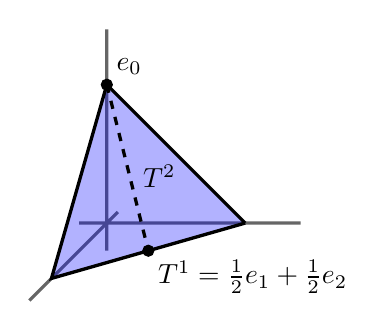
\begin{tikzpicture}[x=1em, y=1em, z=-0.4em, baseline=0.8em]
    \draw[very thick, black!60] 
        (-1,0,0) -- (7,0,0)
        (0,-1,0) -- (0,7,0)
        (0,0,-1) -- (0,0,7);
    \fill[fill=blue, opacity=0.3]
        (5,0,0)--(0,5,0)--(0,0,5)--(5,0,0);
    \draw[very thick, black]
        (5,0,0)--(0,5,0)--(0,0,5)--(5,0,0);
    \draw[dashed, very thick] (0,5,0) -- (2.5,0,2.5);
    \filldraw 
        (0,5,0) circle (2pt) node[anchor=south west] {$e_0$}
        (2,3.5,2.6) node[anchor=north west] {$T^2$}
        (2.5,0,2.5) circle (2pt) node[anchor=north west] {$T^1=\frac{1}{2}e_1+\frac{1}{2}e_2$};
    \end{tikzpicture}$\quad\quad\quad\quad$
    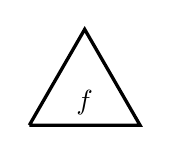
\begin{tikzpicture}[x=4em, y=4em, baseline=0.8em]
    \draw[very thick] (0,0) -- (1,0) -- (0.5, 0.866) -- (0,0);
    \filldraw (0.5, 0.2) node {$f$};
    \end{tikzpicture}$+$
    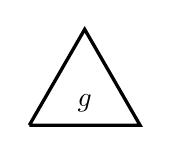
\begin{tikzpicture}[x=4em, y=4em, baseline=0.8em]
    \draw[very thick] (0,0) -- (1,0) -- (0.5, 0.866) -- (0,0);
    \filldraw (0.5, 0.2) node {$g$};
    \end{tikzpicture} $=$
    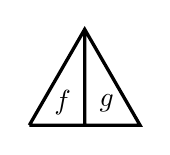
\begin{tikzpicture}[x=4em, y=4em, baseline=0.8em]
    \draw[very thick] (0,0) -- (1,0) -- (0.5, 0.866) -- (0,0)
    (0.5,0)--(0.5, 0.866);
    \filldraw (0.3, 0.2) node {$f$}
    (0.7, 0.2) node {$g$};
    \end{tikzpicture}
\end{center}

Claim. The canonical homomorphism
\[\Z[f:(\ns,\de\ns)\to\pairs]\to \pi_n\pairs^\#,\quad [f]\mapsto[f]\]
factors through a homomorphism
\[\Phi: H_n\left(\frac{C(\S(X,A,n-1))}{C(\S(A))}\right)\to\pi_n\pairs^\#\]
(which is equivalent to saying that $E''\subset E'$).

\begin{claimproof}
We need to show that the two kinds of relations that generate $E''$ are sent to $0$.
\begin{itemize}[label={-}]
    \item If $f:(\ns,\de\ns)\to\pairs$ has image in $A$, we contract $\ns$ onto $e_0$ and postcompose this contraction homotopy with $f$. The result is a pair homotopy from $f$ to a constant map with value $f(e_0)$. So $[f]=[\const_{f(e_0)}]$, which is the zero element in $\pi_n\pairs^\#$.
    \item Now we consider all maps $g:\sx{n+1}\to X$ with $g(\sk_\ni(\sx{n+1}))\subset A$. We want to show that $\sum_0^{n+1}(-1)^i [g\circ(d_i)_*]=0$ in $\pi_n\pairs^\#$.
\end{itemize}

We consider the space $B=\sx{n}\cup_{\sx{n-1}}\dots\cup_{\sx{n-1}}\sx{n}$. It is a quotient space of a disjoint union of $n+2$ copies of $\ns$. If we number these copies from $0$ to $n+1$, we glue the $i$-th copy to the $(i+1)$-st copy by the maps:
\begin{center}
    \begin{tikzcd}
    \sx{\ni} \arrow[d,"(d_i)_*"] \arrow[r,"(d_i)_*"] & \ns_{((i+1)\text{-st})} \\
    \ns_{(i\text{-th})}
    \end{tikzcd}
\end{center}

Informally, $B$ is $\de\sx{n+1}$ "cut open", as shown in the following picture.
\begin{center}
    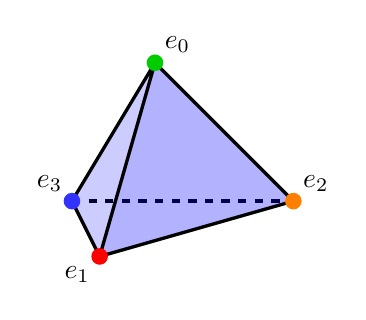
\begin{tikzpicture}[x=1em, y=1em, z=-0.4em, baseline=0.8em]
    \draw[very thick, black, dashed] 
        (-3,0,0) -- (5,0,0);
    \fill[fill=blue, opacity=0.3]
        (5,0,0)--(0,5,0)--(0,0,5)--(5,0,0);
    \fill[fill=blue, opacity=0.2]
        (-3,0,0)--(0,5,0)--(0,0,5)--(-3,0,0);
    \draw[very thick, black]
        (5,0,0)--(0,5,0)
        (0,0,5)--(5,0,0)
        (0,5,0)--(0,0,5)
        (-3,0,0)--(0,5,0)
        (0,0,5)--(-3,0,0);
    \filldraw 
        (0,5,0) circle (2pt) node[anchor=south west] {$e_0$}
        (5,0,0) circle (2pt) node[anchor=south west] {$e_2$}
        (0,0,5) circle (2pt) node[anchor=north east] {$e_1$}
        (-3,0,0) circle (2pt) node[anchor=south east] {$e_3$};
    \fill[red]
        (0,0,5) circle (3pt);
    \fill[blue!80]
        (-3,0,0) circle (3pt);
    \fill[green!80!black]
        (0,5,0) circle (3pt);
    \fill[orange]
        (5,0,0) circle (3pt);
    \end{tikzpicture}$\quad\quad\quad\quad$
    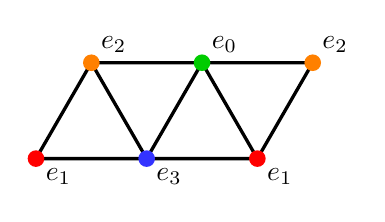
\begin{tikzpicture}[x=4em, y=4em, baseline=0.8em]
    \draw[very thick]
        (0,0) -- (2,0)
        (0,0) -- (0.5, 0.866)
        (1,0) -- (0.5, 0.866)
        (0.5, 0.866) -- (2.5, 0.866)
        (1,0) -- (1.5, 0.866)
        (2,0) -- (1.5, 0.866)
        (2,0) -- (2.5, 0.866);
    \filldraw
        (0,0) node[anchor=north west] {$e_1$}
        (1,0) node[anchor=north west] {$e_3$}
        (2,0) node[anchor=north west] {$e_1$}
        (0.5, 0.866) node[anchor=south west] {$e_2$}
        (1.5, 0.866) node[anchor=south west] {$e_0$}
        (2.5, 0.866) node[anchor=south west] {$e_2$};
    \fill[red]
        (0,0) circle (3pt)
        (2,0) circle (3pt);
    \fill[blue!80]
        (1,0) circle (3pt);
    \fill[green!80!black]
        (1.5, 0.866) circle (3pt);
    \fill[orange]
        (0.5, 0.866) circle (3pt)
        (2.5, 0.866) circle (3pt);
    \end{tikzpicture}
\end{center}
\smallskip
We define $p:B\to\de\sx{n+1}$ by defining the restriction to the $i$-th copy of $\ns$ as $(d_i)_*$. The map $p$ is compatible with the equivalence relation (and hence well defined on $B$) thanks to the simplicial relations:
\[d_i\circ d_i=d_{i+1}\circ d_i\]
The upshot is that $p$ is a quotient map onto $\de\sx{n+1}$.

Since $g$ is defined on all of $\sx{n+1}$, its restriction to $\de\sx{n+1}$ represents the $0$ element in $\pi_n\pairs^\#$.

\[\ns\cong B\xto{p}\de\sx{n+1}\into\sx{n+1}\xto{g}X\]

We apply the homotopy addition theorem (in simplex version) for the maps $\nno{f}{n+1}:\sx{n}\to B=\sx{n}\cup_{\sx{n-1}}\dots\cup_{\sx{n-1}}\sx{n}$, where $f_i$ is the inclusion of the $i$-th copy.
By the HAT:
\[0=[g|_{\de \sx{m+1}}\circ p]=\sum_{i=0}^{m+1}(-1)^i[g\circ (d_i)_*]\]

\end{claimproof}

Let's finish once and for all the proof:
\[H_n\left(\frac{C(\S(X,A,n-1))}{C(\S(A))}\right)\xto{\Phi}\pi_n(X,A)^\#\xto{h^\#}H_n(X,A;\Z)\]
the composite $h^\#\circ\Phi$ is the homomorphism induced by the inclusion $\S(X,A,n-1)\hto \S(X)$, which is an isomorphism. So $\Phi$ is injective. But $\Phi$ is also surjective since it hits all generators. So $\Phi$ is an isomorphism, hence $h^\#$ is an isomorphism.
\end{proof}



\chapter{Fibre Bundles and Fibrations}

\section{Generalities on Fibre Bundles}

A \textbf{fibre bundle} over a space $B$ is a continuous map $\pi:E\to B$ that is locally trivial in the following sense: for every point $b\in B$ there is a space $F$, a neighbourhood $U\subset B$ of $b$ and a homeomorphism such that the following diagram commutes:
\begin{center}
    \begin{tikzcd}
    \pi^{-1}(U) \arrow[dr,"\pi"] \arrow[rr,"\cong"] && U\times F \arrow[dl,"\pr_1"]\\
    & U
    \end{tikzcd}
\end{center}

$B$ is called the \textbf{base}, $E$ the \textbf{total space}, $F$ is the \textbf{fibre}, $\pi$ is the \textbf{projection}, the maps $\pi^{-1}(U)\xto{\cong} U\times F$ the \textbf{local trivialisations}.

If we fix $F$, the set of points $b\in B$ such that $F_b=\pi^{-1}(b)$ is homeomorphic to $F$ is open. So in particular, if $B$ is connected, then all fibres are homeomorphic.

\begin{examples}

Trivial fiber bundles: $\pi=\pr_1:E=B\times F\to B$.

Covering spaces: locally trivial fibre bundle with discrete fiber.

Vector bundles: particular fibre bundles with fibre $\R^n$.

Hopf fibration: $\eta:S^3\to S^2$.

\end{examples}

\begin{remark}

Suppose $\pi:E\to B$ is a locally trivial fibre bundle with fibre $\R^n$. For it to be a \textbf{vector bundle} there must be:
\begin{itemize}[label={-}]
    \item additional structure, as each fibre $F_b=\pi^{-1}(b)$ is given the structure of an $\R$ vector space,
    \item  additional conditions, i.e. the local trivialisation $\pi^{-1}(U)$ are fiberwise linear isomorphisms.
\end{itemize}

An equivalent perspective is the following. Suppose we chose a cover of $B$ by open subsets $\cb{U_i}_{i\in I}$ and local trivializations for each $U_i$, $u_i:\pi^{-1}(U_i)\xto{\cong} U_i\times\R^n$. For each pair of indices $i,j$ the "change of charts"
\[(U_i\cap U_j)\times\R^n\xto{u_i^{-1}}\pi^{-1}(U_i\cap U_j)\xto{u_j}(U_i\cap U_j)\times\R^n\]
is a homeomorphism on the projection to the first factors. So $\Phi=u_j\circ u_i^{-1}$ is of the form
\[(u_j\circ u_i^{-1})(x,v)=(x,\Psi(x,v))\]
for some map $\Psi:(U_i\cap U_j)\times\R^n\to\R^n$. The map $\Phi$ is adjoint to a function
\[U_i\cap U_j\to\homeo(\R^n,\R^n), x\mapsto\Psi(x,-)\]
In a vector bundle, the map factors through $\GL_n(\R)$, the linear automorphisms of $\R^n$.

Several related concepts/refinements of fibre bundles can also be conveniently formulated this way, by specifying a \textbf{structure group}, for example there is a hierarchy:
\begin{itemize}
    \item locally trivial fibre bundles with structure group $\homeo(\R^n,\R^n)$,
    \item smooth bundles with structure group $\diffeo(\R^n,\R^n)$,
    \item vector bundles with structure group $\GL_n(\R^n)$,
    \begin{itemize}
        \item vector bundles can be equipped with an inner product, in which case the structure group is required to be $\text{O}(n)$, 
    \end{itemize}
    \item oriented bundles with structure group $\GL_n^+(\R^n)$,
    \begin{itemize}
        \item oriented vector bundles can be equipped with an inner product, in which case the structure group is required to be $\text{SO}(n)$.
    \end{itemize}
\end{itemize}

\end{remark}

%%% Lecture 7

\section{Hopf Fibration}

\lecture[We construct the thing on the background of Schwede's homepage (Hopf fibration) and we introduce the long exact sequence associated to a fiber bundle (we also use our new toys to compute $\pi_3(S^2)$).]{2021-11-8}

The goals of the following two lectures (which are given by Markus Hausmann, a PhD student of Schwede) are:
\begin{enumerate}
    \item to construct the \textbf{Hopf fibration}, a fibre bundle $\eta:S^3\to S^2$ with fibre $S^1$,
    \item to associate to every fibre bundle $p:E\to B$ a long exact sequence of the form
    \[\cdots\to\pi_n(p^{-1}(b),e)\xto{i_*}\pi_n(E,e)\xto{p_*}\pi_n(B,b)\to\pi_\ni(p^{-1}(b),e)\to\cdots\]
\end{enumerate}

When we are done, we will have as a corollary the computation of our first \textit{really} non-trivial homotopy group.

\begin{corollary}
For every $n\geq 3$ there is an isomorphism $\pi_n(S^3,*)\cong\pi_n(S^2,*)$. In particular, $\pi_3(S^2,*)\cong\Z$, generated by the class of the Hopf fibration.
\end{corollary}

\begin{proof}
For $n\geq3$ we have
\[\cdots\to\pi_n(S^1,*)=0\to\pi_n(S^3,*)\xto{\eta_*}\pi_n(S^3,*)\to\pi_\ni(S^1,*)=0\to\cdots\]
which yields the claim.

In particular, for $n=3$ we get that $\eta_*:\pi_3(S^3,*)\cong\Z\to\pi_3(S^2,*)$ is an isomorphism which sends $[\id_{S^3}]$, generator of $\pi_3(S^3,*)$, to $[\eta\circ\id_{S^3}]=[\eta]$.
\end{proof}

The Hopf fibration is part of a family of fibre bundles.

Let $K=\R$ or $\CC$ and recall the projective spaces:
\[\kpn=(K^{n+1}\sm\cb{0})/K^\times\]
where $x\sim\lambda x$ for all $x,\lambda\in K^\times$. In particular, we have that:
\begin{enumerate}[label={-}]
    \item $\rpn$ is an $n$-dimensional manifold,
    \item $\cpn$ is a $2n$-dimensional manifold.
\end{enumerate}
Moreover, recall that $\rp{1}\cong S^1$ and $\cp{1}\cong S^2$.

We consider now the projections $p:K^{n+1}\sm\cb{0}\to\kpn$.

Let $G$ be a topological group. A principal $G$-bundle is a $G$-space $E$ such that:
\begin{numerate}
    \item for every $e\in E$ the map $G\to Ge=\cb{ge\mid g\in G}$, $g\to ge$, is a homeomorphism,
    \item the quotient map $p:E\to E/G=E/\sim$, where $e\sim ge$ for all $e\in E$, $g\in G$, is a fibre bundle.
\end{numerate}

\begin{example}
The group action of the additive group of the real numbers with the discrete topology on itself (with the standard topology):
\[\R^d\times\R\to\R\]
is an example of free action which does not satisfy property (2).
\end{example}

\begin{proposition}
 For $K=\R$ or $\CC$, the $K^\times$ action on $K^{n+1}\sm\cb{0}$ is a $K^\times$-principal bundle.
\end{proposition}

\begin{proof}
Let $e\in K^{n+1}\sm\cb{0}$. Then the map
\[K^\times\to K^\times e,\ \ \lambda\mapsto\lambda e\]
is continuous and satisfies $\|\lambda_1 e-\lambda_2 e\|=|\lambda_1-\lambda_2|\|e\|$. It follows that the inverse is also continuous.

It remains to show that $K^{n+1}\sm\cb{0}\to \kpn$ is a locally trivial fibre bundle. For $1\leq i\leq n+1$ let $X_i\subset K^{n+1}\sm\cb{0}$ be the subspace of tuples $(x_1,\dots,x_{n+1})$ such that $x_i\neq 0$, i.e. $x_i\in K^\times$. Then $K^{n+1}\sm\cb{0}=\cup_{i=1}^{n+1}X_i$. Let $Y_i=p(X_i)\subset \kpn$. This is open since $p^{-1}(Y_i)=X_i$. We define $u:p^{-1}(Y_i)=X_i\to Y_i\times K^\times$ by $u(x)=(p(x),x_i)$, with inverse
\[u^{-1}([x],\lambda)=(x_1/x_i,\dots,x_{i-1}/x_i,\lambda,x_{i+1}/x_i,\dots,x_{n+1}/x_i).\]
\end{proof}

For $K=\CC$ and $n=1$ this gives a fibre bundle
\[p:\CC^2\sm\cb{0}\cong S^3\to \cp{1}\cong S^2\]
with fibre $\CC^\times\cong S^1$. This is already the Hopf fibration "up to homotopy".

Let $S(K^n)\subset K^n$ be the unit sphere ($(n-1)$-dimensional if $K=\R$, $(2n-1)$-dimensional if $K=\CC$). Further, let $G(K)\subset K^\times$ be the subgroup of elements of norm $1$ ($G(\R)=\cb{\pm1}$, $G(\CC)=S^1$). Then the $K^\times$-action on $K^{n+1}\sm\cb{0}$ restricts to a $G(K)$-action on $S(K^{n+1})$ and the induced map
\begin{center}
    \begin{tikzcd}
    S(K^{n+1})\arrow[r]\arrow[dr] & K^{n+1}\sm\cb{0}\arrow[r] & \kpn \\
    & S(K^{n+1})/G(K)\arrow[ur,swap,"\cong"]
    \end{tikzcd}
\end{center}
is a homeomorphism.

\begin{proposition}
The $G(K)$-action on $S(K^{n+1})$ defines a $G(K)$-principal bundle with base space $\kpn$.
\end{proposition}

\begin{proof}
Let $X_i\subset K^{n+1}\sm\cb{0}$, $Y_i\subset \kpn$ as before. We obtain a homeomorphism
\[v:q^{-1}(Y_i)=S(K^{n+1})\cap X_i\to Y_i\times G(K),\ \ x\mapsto (q(x),x_i/|x_i|).\]
\end{proof}

For $K=\R$ we obtain the covering space $S^n\to\rpn$ we already knew.

For $K=\CC$ we get a fibre bundle $S^{2n+1}\to\cpn$ with fibre $S^1$. For $n=1$ we get the Hopf fibration $\eta:S^3\to S^2$.

\begin{remark}
The Hopf fibration decomposes $S^3$ as a disjoint union of circles, continuously indexed over $S^2$.
It can be shown that any two of them are linked!

Considering $\eta:S^3\to S^2$ and $x_1\neq x_2\in S^2$
\[s:S^3\supset\eta^{-1}(x_1)\times\eta^{-1}(x_2)\to S^2,\ (x,y)\to\frac{x-y}{||x-y||}\]
is continuous. Choosing orientations on $S^2$ and $\eta^{-1}(x_1)\times\eta^{-1}(x_2)\cong S^1\times S^1$, we can consider the mapping degree of $s$. This is an example of an invariant for links called the \textbf{linking number} and it will be $\pm1$ in this case.
\end{remark}\smallskip

\begin{center}\rightnote{Someday I'll really wrap my head around this picture... (but maybe it's just not \textit{that} illuminating?)}
    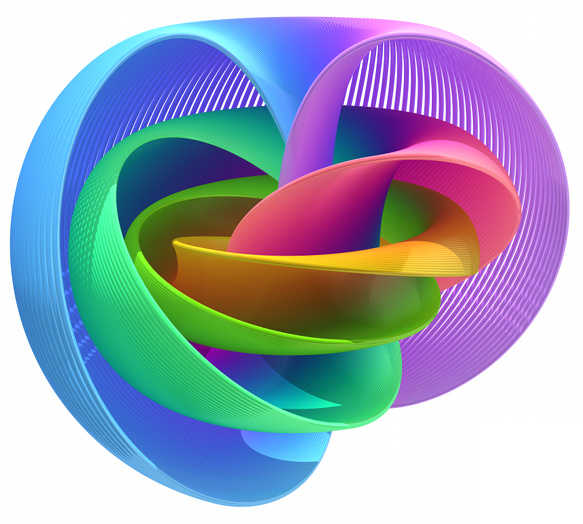
\includegraphics[scale=0.45]{Pictures/HopfFibration.jpg}
\end{center}

\section{The Long Exact Sequence Associated to a Serre Fibration}

We turn now to our second goal. If $p:E\to B$ is a fibre sequence, $b\in B$, $e\in p^{-1}(b)$, then we want to show that there is a long exact sequence of the form:
\[\cdots\to\pi_n(p^{-1}(b),e)\to\pi_n(E,e)\to\pi_n(B,b)\to\cdots\]

\begin{example}
Let $p:E\to B$ be a covering space. We get a long exact sequence (assuming $E$ is connected):
\[\cdots\to\pi_n(p^{-1}(b),e)=0\to\pi_n(E,e)\to\pi_n(B,b)\to\pi_\ni(p^{-1}(b),e)=0\to\cdots\]
\[\cdots\to 0 \to\pi_1(E,e)\to\pi_1(B,b)\to\pi_0(p^{-1}(b),e)\to 0\]

This amounts to the known statements that $p_*:\pi_1(E,e)\to\pi_1(B,b)$ is injective (and that the fiber can be identified, via path lifting, with the set of cosets of $p_*\pi_n(E,e)$ in $\pi_1(B,b)$) and that $p_*:\pi_n(E,e)\to\pi_n(B,b)$ is an isomorphism for $n\geq 2$. Both facts have been already proven using the lifting properties of covering spaces.\rightnote{He adds a reminder on map lifting here.}
\end{example}

Let $p:E\to B$ be a continuous map. A \textbf{test situation} for the homotopy lifting property (HLP) consists of a space $X$ and a commutative square:
\begin{center}
    \begin{tikzcd}
    X \arrow[d,"i_0"] \arrow[r,"f"] & E \arrow[d,"p"] \\
    X\times[0,1] \arrow[r,"H"] & B
    \end{tikzcd}
\end{center}

A solution to the test situation is a map $\til H:X\times[0,1]\to E$
 such that $p\circ\til H=H$ and $\til H\circ i_0=f$.
 
 there is also a relative version: a pair of spaces $\pairs$ and a commutative diagram:
\begin{center}
    \begin{tikzcd}
    X\times\cb{0}\cup(A\times[0,1]) \arrow[d, hook,"i_0"] \arrow[r,"f"] & E \arrow[d,"p"] \\
    X\times[0,1] \arrow[r,"H"] & B
    \end{tikzcd}
\end{center}

A solution is again a map $\til H:X\times[0,1]\to E$ such that $p\circ\til H=H$ and $\til H\circ i_0=f$.

A map $p:E\to B$ is called a \textbf{Hurewicz fibration} if it has the HLP with respect to all $X$ and all absolute test-situations for $X$.

A map $p:E\to B$ is called a \textbf{Serre fibration} if it has the HLP with respect to every CW-complex $X$ and all absolute test-situations for $X$.

For the proof of the existence of the long exact sequence associated to a fibre bundle we need two intermediate results.

\begin{proposition**}
Let $p:E\to B$ be a Serre fibration, $Y\subset B$ a subspace and $x\in p^{-1}(Y)$. Then the projection induces an isomorphism (for $n\geq 1$):
\[p_*:\pi_n(E,p^{-1}(Y),*)\xto{\cong}\pi_n(B,Y,p(x))\]
\end{proposition**}

\begin{corollary**}
Let $Y=\cb{b}$. We get a long exact sequence:
\[\cdots\to\pi_n(p^{-1}(b),x)\to\pi_n(E,x)\to\pi_n(E,p^{-1}(b),x)\cong\pi_n(B,b)\to\cdots\]
\end{corollary**}

\begin{theorem**}
Every fiber bundle is a Serre fibration.
\end{theorem**}

%%% Lecture 8

\lecture[We actually prove the story about the long exact sequence associated to a fibre bundle.]{2021-11-10}

Before we get to the two promised lemmas, we prove an auxiliary one.\rightnote{\Attention\ Didn't sleep much the night before this one, I hope I didn't type anything too stupid!}

\begin{lemma}\label{lemma:equivalent-HCP}
Let $p:E\to B$ be a map. The following are equivalent:
\begin{numerate}
\item $p$ is a Serre fibration,
\item $p$ has the absolute HLP for $D^n$ for all $n$,
\item $p$ has the relative HLP for $(D^n,\de D^n)$ for all $n$,
\item $p$ has the relative HLP for all relative CW-complexes.
\end{numerate}
\end{lemma}

\begin{proof}

$(1)\implies(2)$ This is true because $D^n$ is a CW-complex.

$(2)\implies(3)$ The space pairs $(D^n\times[0,1],D^n\times\cb{0})$ and $(D^n\times[0,1],D^n\times\cb{0}\cup\de D^n\times[0,1])$ are homeomorphic, hence any test situation for one HLP can be translated into a test situation for the other, and similarly for the solutions.

$(3)\implies(4)$ Let $(X,X')$ be a relative CW-complex. Consider the test situation:
\begin{center}
    \begin{tikzcd}
    X\times\cb{0}\cup X'\times[0,1] \arrow[d] \arrow[r,"f"] & E \arrow[d,"p"] \\
    X\times[0,1] \arrow[r] & B
    \end{tikzcd}
\end{center}

We first assume that $X=X'\cup_{\de D^n}D^n$ is obtained from $X'$ by attaching a single cell, with characteristic map $\alpha:D^n\to X$.

We obtain:

\begin{center}
    \begin{tikzcd}[row sep=huge]
    D^n\times\cb{0} \cup\de D^n\times[0,1] \arrow[d] \arrow[r] & X\times\cb{0} \cup X'\times[0,1] \arrow[d] \arrow[r,"f"] & E \arrow[d,"P"] \\
    D^n\times[0,1] \arrow[urr,dashed,crossing over,shift right,"H'"] \arrow[r,swap,"\alpha\times\id_{[0,1]}"] & X\times[0,1] \arrow[r,swap,"H"] & B
    \end{tikzcd}
\end{center}

By assumption, there exists a lift $H'$ as in the diagram.

Then the desired solution is
\[X\times[0,1]=(X'\times[0,1])\cup_{\de D^n\times[0,1]}D^n\times[0,1]\xto{f\cup H'}E.\]

The case where $(X,X')$ has finitely many relative cells follows by induction, the infinite case by passing to the colimit.

$(4)\implies(1)$ This is the special case $(X,\emptyset)$.

\end{proof}

\begin{remark}
Note: CW-complexes are colimits of their skeleta.

\begin{center}
    \begin{tikzcd}
    \sk_n X\times[0,1] \arrow[r] \arrow[d,hook] & E \\
    \sk_{n+1}X\times[0,1] \arrow[ur,]
    \end{tikzcd}
\end{center}

We have $X\cong\colim_n\sk_n X$ and $X\times[0,1]\cong\colim_n(\sk_n X\times[0,1])$.
\end{remark}

\begin{proposition}
Let $p:E\to B$ be a Serre fibration, $Y\subset B$ and $x\in p^{-1}(Y)$. Then $p$ induces an isomorphism
\[p_*\pi_n(E,p^{-1}(Y),x)\xto{\cong}\pi_n(B,Y,p(x))\]
for all $n\geq1$.
\end{proposition}

\begin{proof}\ 

Surjectivity. Let $[\beta]\in\pi_n(B,Y,p(x))$ be represented by $\beta(I^n,\de I^n,s_0)\to(B,Y,p(x))$ with $s_0=(0,\dots,0)$.
\begin{center}
    \(
    \begin{tikzcd}
    
\begin{tikzpicture}[x=2em, y=2em, baseline=0.7em]
        \draw[very thick, black!30] (0,0)--(1,0)--(1,1)--(0,1)--(0,0);
        \filldraw (0,0) circle (2pt);
    \end{tikzpicture}
    \ar[r, hook]\ar[d]
    & 
    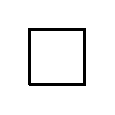
\begin{tikzpicture}[x=2em, y=2em, baseline=0.7em]
        \draw[very thick] (0,0)--(1,0)--(1,1)--(0,1)--(0,0);
    \end{tikzpicture} 
    \ar[r, hook]\ar[d]
    &
    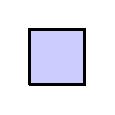
\begin{tikzpicture}[x=2em, y=2em, baseline=0.7em]
        \filldraw[very thick, fill=blue!20] (0,0)--(1,0)--(1,1)--(0,1)--(0,0);
    \end{tikzpicture}
    \ar[d]\\
    p(x)\ar[r, hook]&Y\ar[r, hook]&B
    \end{tikzcd}
    \)
\end{center}


This already looks like a homotopy but we need to lift $\beta|_{I^\ni\times\cb{0}}$. There's different ways to go about this, for example repeated applications of the HEP would work, but since we're working with a contractible space, there's an easier and faster way.

Applying the HEP first to the relative CW-complex $(\de I^n,I^\ni\times\cb{0})$ (for maps into $Y$), and second for the relative CW-complex $\pair$ mapping into $B$, we can replace $\beta$ by an homotopic map $\beta'$ which sends all of $I^\ni\times\cb{0}$ to $p(x)$.

\begin{center}
    \(
    \begin{tikzcd}
    
\begin{tikzpicture}[x=2em, y=2em, baseline=0.7em]
        \draw[very thick, black!30] (0,0)--(1,0)--(1,1)--(0,1)--(0,0);
        \draw[very thick]
        (0,0)--(1,0);
    \end{tikzpicture}
    \ar[r, hook]\ar[d]
    & 
    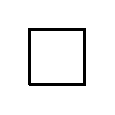
\begin{tikzpicture}[x=2em, y=2em, baseline=0.7em]
        \draw[very thick] (0,0)--(1,0)--(1,1)--(0,1)--(0,0);
    \end{tikzpicture} 
    \ar[r, hook]\ar[d]
    &
    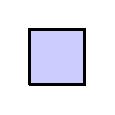
\begin{tikzpicture}[x=2em, y=2em, baseline=0.7em]
        \filldraw[very thick, fill=blue!20] (0,0)--(1,0)--(1,1)--(0,1)--(0,0);
    \end{tikzpicture}
    \ar[d]\\
    p(x)\ar[r, hook]&Y\ar[r, hook]&B
    \end{tikzcd}
    \)
\end{center}

The constant map $c_{p(x)}:I^\ni\times\cb{0}\to Y$ has a canonical lift to $E$ via the constant map $c_x:I^\ni\times\cb{0}\to p^{-1}(Y)$. Hence we obtain:
\begin{center}
    \begin{tikzcd}[column sep=large]
    I^\ni\times\cb{0} \arrow[d] \arrow[r,"c_x"] & E \arrow[d,"p"] \\
    I^n \arrow[r,swap,"\beta'"] \arrow[ur,dashed,"\exists\til\beta"] & B
    \end{tikzcd}
\end{center}
Since $p$ is a Serre fibration, there exists $\til\beta:I^n\to E$ such that $\til\beta|_{I^\ni\times\cb{0}}=c_x$ (in particular $\til\beta(s_0)=x$) and $p\circ\til\beta=\beta'$ (in particular $\til\beta(\de I^n)\subset p^{-1}(Y)$). Hence $\til\beta$ represents an element $[\til\beta]$ of $\pi_n(E,p^{-1}(Y),x)$, which by construction maps to $[\beta']=[\beta]$ under $p_*$.

Injectivity. Let $\alpha_1,\alpha_2:(I^n,\de I^n,s_0)\to(E,p^{-1}(Y),x)$ represent elements of $\pi_n(E,p^{-1}(Y),x)$ which are sent to the same element under $p_*$. Then there exists a homotopy of triple maps $H:I^n\times I\to B$ from $p\circ\alpha_1$ to $p\circ\alpha_2$.\vspace{-0.2cm}
\[
\begin{tikzcd}[column sep = huge]
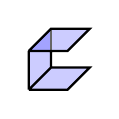
\begin{tikzpicture}[x = 1.4em, y = 1.4em, z = 0.8em, baseline = 0.4em]
    \begin{scope}[fill=blue, opacity=0.2]
    \fill
    (0,0,0) -- (0,1,0) -- (0,1,1) -- (0,0,1) -- (0,0,0);
    \fill
    (0,0,0) -- (1,0,0) -- (1,0,1) -- (0,0,1) -- (0,0,0);
    \fill
    (0,1,0) -- (1,1,0) -- (1,1,1) -- (0,1,1) -- (0,1,0);
    \end{scope}
    \begin{scope}[thick]
    \draw[black!60]
    (0,0.4,1) -- (0,1,1);
    \draw
    (0,0,1) -- (0,0.45,1)
    (0,0,0) -- (0,1,0)
    (0,0,0) -- (1,0,0) -- (1,0,1) -- (0,0,1) -- (0,0,0)
    (0,1,0) -- (1,1,0) -- (1,1,1) -- (0,1,1) -- (0,1,0);
    \end{scope}
\end{tikzpicture}
\ar[r, "\alpha_1\cup c_x\cup\alpha_2"] \ar[d] & E \ar[d, " p"]\\
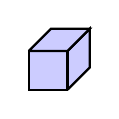
\begin{tikzpicture}[x = 1.4em, y = 1.4em, z = 0.8em, baseline = 0.4em]
    \begin{scope}[fill=blue!20, thick]
    \filldraw
    (1,0,0) -- (1,1,0) -- (1,1,1) -- (1,0,1) -- (1,0,0);
    \filldraw
    (1,0,0) -- (1,1,0) -- (0,1,0) -- (0,0,0) -- (1,0,0);
    \filldraw
    (0,1,0) -- (1,1,0) -- (1,1,1) -- (0,1,1) -- (0,1,0);
    \end{scope}
\end{tikzpicture}
\ar[r, "H"'] \ar[ur, dashed] & B
\end{tikzcd}
\]


Again we can assume that $\alpha_1(I^\ni\times\cb{0})=\alpha_2(I^\ni\times\cb{0})=\cb{x}$. In addition we can assume that $H$ sends $(I^\ni\times\cb{0})\times I$ constantly to $p(x)$. We again lift $c_{p(x)}$ to $c_x$ and view $\alpha_1$ and $\alpha_2$ as lifts of $H$ on the subspace $I^\ni\times\cb{0}\times\cb{0}\cup I^\ni\times\cb{0}\times\cb{1}$. Since $(I^\ni\times\cb{0}\times I,I^\ni\times\cb{0}\times\cb{0}\cup I^\ni\times\cb{0}\times\cb{1})$ is a relative CW-complex, we can apply the relative HLP to lift $H$ to a map $\til H:I^n\times I\to E$, giving a relative homotopy from $\alpha_1$ to $\alpha_2$.
\end{proof}

\begin{theorem}
Every fibre bundle is a Serre fibration.
\end{theorem}

\begin{proof}
Let $p:E\to B$ be a fibre bundle and a lifting problem
\begin{center}
    \begin{tikzcd}
    X\times\cb{0} \arrow[r,"f"] \arrow[d] & E \arrow[d,"p"] \\
    X\times I \arrow[r,"H"] & B
    \end{tikzcd}
\end{center}

Easy case. Let $p$ be globally trivial, i.e. of the form $\pr_B:B\times F\to B$ for some space $F$. Then we have
\begin{center}
    \begin{tikzcd}[column sep=large]
    X\times\cb{0} \arrow[r,"{(f_1, f_2)}"] \arrow[d] & B\times F \arrow[d,"\pr_B"] \\
    X\times I \arrow[r,swap,"H"] \arrow[ur,dashed,"\til H"] & B
    \end{tikzcd}
\end{center}
We can define a lift $\til H$ explicitly via $\til H(x,t)=(H(x,t),f_2(x))$ (this works for any space $X$).

General case. We have to glue local lifts together systematically.

By lemma \ref{lemma:equivalent-HCP}, it suffices to check the HLP for disks $D^n$, or equivalently for cubes $I^n$. Hence we are given:
\begin{center}
    \begin{tikzcd}
    I^n\times\cb{0} \arrow[r,"f"] \arrow[d] & E \arrow[d,"p"] \\
    I^n\times I \arrow[r,"H"] & B
    \end{tikzcd}
\end{center}

Let $\cb{U_i}_{i\in I}$ be an open covering of $B$, such that $p^{-1}(U_i)\xto{p}U_i$ is a trivial fibre bundle for all $i$. Pulling back along $H$, we get an open cover of $I^n\times I$. By Lebesgue's lemma, we can divide $I^n\times I$ into smaller cubes of side length $1/k$, such that each cube is contained in some $p^{-1}(U_i)$.\rightnote{The drawing is an explanation of how "row by row" is fine and otherwise not: \textcolor{red}{add explanation!}}
\begin{center}
    \(
    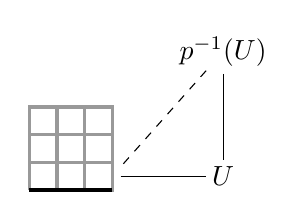
\begin{tikzpicture}[x=1em, y=1em, baseline=1em]
        \draw[very thick, black!40]
            (0,0)--(3,0)--(3,3)--(0,3)--(0,0)
            (1,0)--(1,3) (2,0)--(2,3)
            (0,1)--(3,1) (0,2)--(3,2);
        \draw[very thick] (0,0)--(3,0);
        \draw[-{\tip}, shorten <= 3pt, shorten >= 6pt] (3,.5)--(7,.5);
        \draw[-{\tip}, shorten <= 8pt, shorten >= 6pt] (7,5)--(7,.5);
        \draw[-{\tip}, shorten <= 6pt, shorten >= 8pt, dashed] (3,.5)--(7,5);
        \filldraw 
            (7,0.5) node{$U$}
            (7,5) node{$p^{-1}(U)$};
    \end{tikzpicture}
    \quad\leadsto\quad
    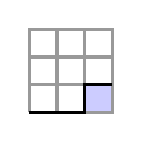
\begin{tikzpicture}[x=1em, y=1em, baseline=1em]
        \fill[blue!20] (2,0)--(2,1)--(3,1)--(3,0);
        \draw[very thick, black!40]
            (0,0)--(3,0)--(3,3)--(0,3)--(0,0)
            (1,0)--(1,3) (2,0)--(2,3)
            (0,1)--(3,1) (0,2)--(3,2);
        \draw[very thick] (0,0)--(2,0)--(2,1)--(3,1);
    \end{tikzpicture}
    \quad\leadsto\cdots\leadsto\quad
    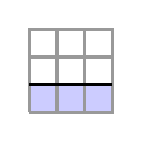
\begin{tikzpicture}[x=1em, y=1em, baseline=1em]
        \fill[blue!20] (0,0)--(0,1)--(3,1)--(3,0);
        \draw[very thick, black!40]
            (0,0)--(3,0)--(3,3)--(0,3)--(0,0)
            (1,0)--(1,3) (2,0)--(2,3)
            (0,1)--(3,1) (0,2)--(3,2);
        \draw[very thick] (0,1)--(3,1);
    \end{tikzpicture}
    \quad\leadsto\cdots\leadsto\quad
    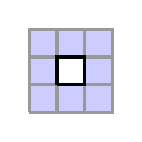
\begin{tikzpicture}[x=1em, y=1em, baseline=1em]
        \fill[blue!20] (0,0)--(0,3)--(3,3)--(3,0);
        \draw[very thick, black!40]
            (0,0)--(3,0)--(3,3)--(0,3)--(0,0)
            (1,0)--(1,3) (2,0)--(2,3)
            (0,1)--(3,1) (0,2)--(3,2);
        \filldraw[very thick, fill=white] (1,1)--(2,1)--(2,2)--(1,2)--(1,1);
    \end{tikzpicture}
    \quad\leadsto \Attention
    \)
\end{center}\medskip

We can then extend $H$ iteratively over the smaller cubes "row by row". In every situation this amounts to choosing a solution to the relative lifting problem for a globally trivial fibre bundle.

\end{proof}

\begin{remark}
Not every fibre bundle is a Hurewicz fibration (but actual counter-examples are complicated). A sufficient condition is that the base space be paracompact.
\end{remark}

\begin{remark}

An interesting question: are lifting of homotopies unique? It turns out that they are unique up to homotopy!
\begin{center}
    \begin{tikzcd}[column sep=large]
    X\times\cb{0} \arrow[r] \arrow[d] & E \arrow[d,"p"] \\
    X\times I \arrow[r] \arrow[ur,dashed,"\til H_1", "\til H_2"'] & B
    \end{tikzcd}\qquad
    \begin{tikzcd}
    X\times I\times\cb{0} \cup X\times I\times\cb{1} \arrow[r] \arrow[d] & E \arrow[d,"p"] \\
    X\times I\times I \arrow[r] & B
    \end{tikzcd}
\end{center}\normalmarginpar\todo{I wasn't paying attention, it might be interesting to reconstruct the argument!}

\end{remark}

%%% Lecture 9

\section{More on Fibre Bundles and Fibrations}

\lecture[Some more fibre bundles/fibrations stuff. Prof. Schwede suggests that we take the categorical red pill. Shout-out to the category of compactly generated spaces (without definition). We introduce the compact-open topology.]{2021-11-15}

Prof. Schwede is back!

\begin{theorem}
Let $p:E\to B$ be a continuous map, with path-connected base.
\begin{numerate}
    \item If $p$ is a Hurewicz fibration, then any two fibers of $p$ are homotopy equivalent.
    \item If $p$ is a Serre fibration, then any two fibres which are CW-complexes are homotopy equivalent.
\end{numerate}
\end{theorem}

\begin{proof}
Let $b_0,b_1\in B$ be points, set $F_0=p^{-1}(b_0),F_1=p^{-1}(b_1)$.

Let $\omega:[0,1]\to B$ be a path from $b_0$ to $b_1$. Choose homotopies $H$ and $K$ as liftings in the followings diagrams:
\begin{center}
\begin{tikzcd}[column sep=large]
F_0\times 0 \arrow[r,"\incl"] \arrow[d,hook] & E \arrow[d,"p"] \\
F_0\times[0,1] \arrow[ur,dashed,"H"] \arrow[r,"\omega\circ\pr_2"] & B
\end{tikzcd}\qquad
\begin{tikzcd}[column sep=large]
F_1\times 0 \arrow[r,"\incl"] \arrow[d,hook] & E \arrow[d,"p"] \\
F_1\times[0,1] \arrow[ur,dashed,"K"] \arrow[r,"\bar\omega\circ\pr_2"] & B
\end{tikzcd}
\end{center}

where $\bar\omega(t)=\omega(1-t)$ is the inverse path.

We set $f=H(-,1):F_0\to F_1$ and $g=K(-,1):F_1\to F_0$.

Let $L:[0,1]\times[0,1]\to B$ be a homotopy, relative $\cb{0,1}$, from $\omega\times\bar\omega$ (the concatenated path) to $\const_{b_0}$.
\[L(-,0)=\omega\times\bar\omega,\]
\[L(-,1)=\const_{b_0}\]
\[L(0,t)=L(1,t)=b_0\]

Choose another lifting in the following diagram:

\begin{center}
    \begin{tikzcd}[column sep=huge]
    F_0\times((0\times I)\cup(I\times 0)\cup(1\times I))\times 0 \arrow[r] \arrow[d,hook] & E \arrow[d,"p"] \\

    F_0\times[0,1]\times[0,1] \arrow[ur,dashed,swap,"\bar L"] \arrow[r,swap,"L\circ\pr_{2,3}"] & B
    \end{tikzcd}
\end{center}
where the upper arrow is $(\const_{\incl}\,\cup\, H\times(K\circ(f\times\id))\,\cup\,\const_{g\circ f})$.\smallskip

\begin{center}
    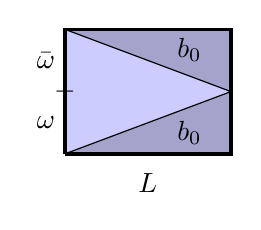
\begin{tikzpicture}[x=1.5em, y=1.5em, baseline=2.1em]
    \filldraw[very thick, fill=blue!20] (0,0)--(0,3)--(4,3)--(4,0)--(0,0);
    \draw (0,0)--(4,1.5)--(0,3);
    \filldraw[fill = black, opacity = 0.2] (0,0)--(4,1.5)--(0,3)--(4,3)--(4,0)--(0,0);
    \filldraw
    (0,.75) node[anchor=east]{$\omega$}
    (0,2.25) node[anchor=east]{$\bar\omega$}
    (0,1.5) node {$-$}
    (3,2.5) node {$b_0$}
    (3,0.5) node {$b_0$}
    (2,-0.7) node{$L$};
    \end{tikzpicture}
    \hspace{2cm}
    \(\displaystyle
    \begin{tikzcd}[column sep=huge]
    F_0\times
        
\begin{tikzpicture}[x=1em, y=1em, baseline=0.2em]
        \draw[very thick] (1,0)--(0,0)--(0,1)--(1,1);
        \end{tikzpicture}
    \arrow[r] \arrow[d,hook] & E \arrow[d,"p"] \\
    F_0\times
        
\begin{tikzpicture}[x=1em, y=1em, baseline=0.2em]
        \filldraw[very thick, fill=blue!20] (1,0)--(0,0)--(0,1)--(1,1)--(1,0);
        \end{tikzpicture}
    \arrow[ur,dashed,swap,"\bar L"] \arrow[r,swap,"L\circ\pr_{2,3}"] & B
    \end{tikzcd}\)
\end{center}

\vspace{-0.1cm}
Then we can set $G=\bar L(-,-,1):F_0\times[0,1]\to E$ to obtain a homotopy from $\incl:F_0\into E$ to $\incl\circ g\circ f:F_0\to E$.

Since $p\circ G=\const_{b_0}$, this homotopy $G$ takes place inside $F_0$.

So $G$ is a homotopy from $\id_{F_0}$ to $g\circ f$. Reversing the roles of $b_0$ with $b_1$, $F_0$ with $F_1$ and $f$ with $g$ yields a homotopy from $\id_{F_1}$ to $f\circ g$.
\end{proof}

\unnumpar{Induced fibres bundles/fibrations}

We construct the pullback bundle\rightnote{This construction is also called base change sometimes.}. Let $p:E\to B$ and $\beta:B'\to B$ be continuous maps. The pullback is \[E'=B'\times_B E=\cb{(b',e)\in B'\times E\mid \beta(b')=p(e)}\]
with subspace topology of the product topology.

\begin{center}
    \begin{tikzcd}
    &[-6ex] (b',e) \arrow[r,mapsto] & e \\[-4ex]
    (b',e) \arrow[d,mapsto] & B'\times_B E \arrow[d,dashed,"p'"] \arrow[r,dashed,"\beta'"] & E \arrow[d,"p"] \\
    
    b' & B' \arrow[r,"\beta"] & B
    \end{tikzcd}
\end{center}

This is a pullback in the sense of category theory, i.e. the following universal property holds: for all spaces $A$ and continuous maps $\alpha:A\to B'$ and $\epsilon:A\to E$ such that $\beta\alpha=p\epsilon$, there is a unique continuous map $\delta:A\to B'\times_B E$ such that $\beta'\delta=\epsilon$ and $\alpha\delta=p'$ (namely the map: $\delta(a)=(\alpha(a),\epsilon(a))$).
\begin{center}
    \begin{tikzcd}
    A \arrow[dr,dashed,"\exists!\delta"] \arrow[drr,bend left,"\epsilon"] \arrow[ddr,bend right,"\alpha"] & & \\
     & B'\times_B E \arrow[d,"p'"] \arrow[r,"\beta'"] & E \arrow[d,"p"] \\
    
     & B' \arrow[r,"\beta"] & B
    \end{tikzcd}
\end{center}

\begin{example}[Restriction bundle]
Suppose $B'$ is a subspace of $B$ and $\beta:B'\to B$ the inclusion. Then
\[B'\times_B E\cong p^{-1}(B')\]
with homeomorphism given by
\[(b',e)\mapsto e\]
\[(p(e),e)\mapsfrom e.\]
\end{example}

\begin{example}[A pretty stupid one]
I lost the explanation, but take it as a little rebus:
\begin{center}
    \begin{tikzcd}
    B'\amalg B' \arrow[d] \arrow[r] & B' \arrow[d] \\
    *\amalg* \arrow[r] & *
    \end{tikzcd}
\end{center}
\end{example}
In general taking the constant map $\beta:B'\to B$ to a point $b\in B$ will yield as the pullback bundle the trivial bundle $B'\times p^{-1}(b)$.

\begin{theorem}
Let $p:E\to B$ and $\beta:B'\to B$ be continuous maps.
\begin{itemize}
    \item[(i)] If $p$ is a fibre bundle, then so is $p':B'\times_B E\to B'$.
    \item[(ii)] If $p$ is a Hurewicz fibration, then so is $p'$.
    \item[(iii)] If $p$ is a Serre fibration, then so is $p'$.
\end{itemize}
\end{theorem}

\begin{proof}\rightnote{\emph{\enquote{You take the blue pill — the story ends, you wake up in your bed and believe whatever you want to believe. You take the red pill — you stay in Wonderland, and I show you how deep the rabbit hole goes.}}}There's two reasonable proofs of the first fact, one direct, one categorical. The Professor seems to be suggesting a blue pill/red pill situation (with the categorical version being \emph{\enquote{much more transparent}} to him).

(i) Consider any point $a\in B'$. There is a open neighbourhood $U$ of $\beta(a)$ in $B$ and a local trivialization, i.e. a homeomorphism $\psi:p^{-1}(U)\to U\times F$ for one space $F$ (over $U$).

We argue that $p':B'\times_B E\to B'$ is trivializable over $V=\beta^{-1}(U)$ with the same fibre $F$.

The following are mutually inverse homeomorphisms:
\begin{align*}
    (p')^{-1}(V)&\xleftrightarrow{\ \cong\ }V\times F\\
    (b',e)&\ \,\mapsto\ (b',\psi_2(\beta(b')))\\
    (b',\psi^{-1}(\beta(b'),f))&\ \,\mapsfrom\ (b',f)
\end{align*}

Categorical proof: pullbacks are transitive.

In any category $\Cc$, we consider a commutative diagram:
\begin{center}
    \begin{tikzcd}[column sep={8em,between origins}]
    B''\times_B E \arrow[d] \arrow[r] & B'\times_B E \arrow[d,"p'"] \arrow[r,"\beta'"] & E \arrow[d] \\
    
    B'' \arrow[r] & B' \arrow[r,"\beta"] & B
    \end{tikzcd}
\end{center}

If both squares are pullbacks, then the composite square is also a pullback. Symbolic notation:
\[B''\times_B E\cong B''\times_{B'}(B'\times_B E).\]

Hence we have:
\[(p')^{-1}(V)=V\times_{B'}(B'\times_B E)\cong V\times_B E = V\times_U(U\times_B E)\cong V\times_U(U\times F)\cong V\times F.\]

(ii)+(iii) We show: whenever $p:E\to B$ has the HPL for some space $X$, then $p':B'\times_B E\to B'$ also has the HLP for $X$.

Consider a lifting square on the left:
\begin{center}
    \begin{tikzcd}[column sep=large,row sep=huge]
    X\times0 \arrow[d,hook] \arrow[r,"f"] & B'\times_B E \arrow[d,"p'" near end] \arrow[r,"\beta'"] & E \arrow[d,"p"] \\
    
    X\times[0,1] \arrow[ur,dashed,bend left=20,blue,"\bar K"] \arrow[urr,dashed,crossing over,red, "K" near start] \arrow[r,"H"'] & B' \arrow[r,"\beta"'] & B
    \end{tikzcd}
\end{center}

There is a homotopy $K:X\times[0,1]\to E$ so that $p\circ K=\beta\circ H$ and $K(-,0)=\beta'\circ f$.

The universal property of the pullback provides a unique continuous map
\[\bar K:X\times[0,1]\to B'\times_B E\]
such that $p'\circ \bar K=H$ and $\beta'\circ\bar K=K$.

Two continuous maps $f,\,\bar K(-,0):X\times0\to B'\times_B E$ compose in the same way with $p'$ and with $\beta'$. The uniqueness part of the universal property then forces $f=\bar K(-,0)$.
\end{proof}

\chapter{Mapping Spaces}

\section{Compact-open Topology}

Our aim: to define and study a specific topology on $Z^X=\cb{f:X\to Z\text{ continuous}}.$

We would like the "exponential law" to hold: the map
\begin{align*}
    Z^{X\times Y}&\to(Z^X)^Y\\
    (f:X\times Y\to Z)&\mapsto \cb{y\mapsto f(-,y)}
\end{align*}
should be a homeomorphism.

Unfortunately, it is not. At least not in general, but the good news is that it is whenever $Y$ is Hausdorff and $X$ locally compact.

\begin{remark}
There is a way to arrange the exponential law in complete generality: work in the full subcategory $CG$ of compactly generated spaces. Then $CG$ is a cartesian closed category, i.e. it has finite products and for all $X\in\operatorname{ob}(G)$
\[-\times X:CG\to CG\]
has a right adjoint, written $Z\mapsto Z^X$.

Watch out: the product in $CG$ is not always the usual product topology!

Some examples of classes of spaces in $CG$ are:
\begin{itemize}[label={-}]
    \item every locally compact Hausdorff spaces,
    \item every CW-complex,
    \item every manifold is in $CG$,
    \item the realization of every simplicial set,
    \item for two CW-complexes $X$ and $Y$, the product in $CG$, $X\times_{CG}Y$, is again a CW-complex.
    \item for all simplicial sets $A,B$, the canonical map:
    \[|A\times B|\to|A|\times_{CG}|B|\]
    is a homeomorphism.
\end{itemize}
\end{remark}

Enter: the compact-open topology. For spaces $X$ and $Z$, write $Z^X$ for the set of continuous maps $f:X\to Z$. Let $K$ be a compact subset of $X$ and let $O$ be an open subset of $Z$. Set:
\[W(K,O)=\cb{f\in Z^X:f(K)\subset O}\subset Z^X.\]

The \textbf{compact-open topology} on $Z^X$ is the topology generated by the sets $W(K,O)$ with $K\subset X$ compact and $O\subset Z$ open, i.e. these sets form a subbasis of the compact-open topology.

\begin{theorem}
Let $X$ be a compact space and $(Z,d)$ a metric space.
\begin{numerate}
\item There is a metric on $Z^X$, defined as:
\[d(g_1,g_2)=\sup_{x\in X}d(g_1(x),g_2(x)),\text{ for }g_1,g_2\in Z^X.\]
called the supremum metric.
\item The compact-open topology on $Z^X$ coincides with the metric topology of the supremum metric.
\end{numerate}
\end{theorem}

\begin{proof}
(1) Omitted (see \cite[Proposition A.13]{Hatcher}.

(2) \enquote{$\subset$}: compact-open is metrically open.

It suffices to show that the generating sets $W(K,O)$ are metrically open. Fix $K\subset X$ compact, $O\subset Z$ open and $f\in W(K,O)$, i.e. $f(K)\subset O$. Then $C=Z\sm O$ is a closed subset of $Z$ and $f(x)\not\in C$ for all $x\in K$ (hence $d(f(x),C)>0$ for all $x\in K$). Since $K$ is compact, $\epsilon=\inf_{x\in K}d(f(x),C)>0$
is positive.
We claim that $B_{\sup}(f,\epsilon)\subset W(K,O)$.

Let $g\in Z^X$ be such that $d(f,g)<\epsilon$. Then $d(f(x),g(x))<\epsilon$ for all $x\in K$, hence:
\[d(f(x),g(x))\leq d(f(x),C),\]
so $g(x)\in O=Z\sm C$. Therefore $g(K)\subset O$, so $g\in W(K,O)$.

\enquote{$\supset$}: metrically open is compact-open.

Let $A\subset Z^X$ be open in the sup-topology, $f\in A$. We will construct finitely many compact sets $K_i$ in $X$ and open sets $O_i$ in $Z$ so that:
\[f\in W(K_1,O_1)\cap\dots\cap W(K_m,O_m)\subset A.\]

Since $A$ is open in the sup-topology, there is an $\epsilon>0$ so that $A$ contains the $\epsilon$-ball around $f$.

For $x\in X$ the set $f^{-1}(B(f(x),\epsilon/5))$ is an open neighbourhood of $x$ in $X$. Since $X$ is compact\rightnote{Note: compact spaces, meaning quasi-compact \textit{and} Hausdorff, are locally compact, but quasi-compact spaces may not be!}, this contains a compact neighbourhood $K_x$ of $x$. Since $X$ is compact, there are finitely many $x_1,\dots,x_m$ such that $X=K_{x_1}\cup\dots\cup K_{x_m}$.
Set $K_i:=K_{x_i}$ and $O_i:=$ open $\epsilon/5$-neighbourhood of $f(K_i)$ in $Z$.

\begin{center}\scriptsize
    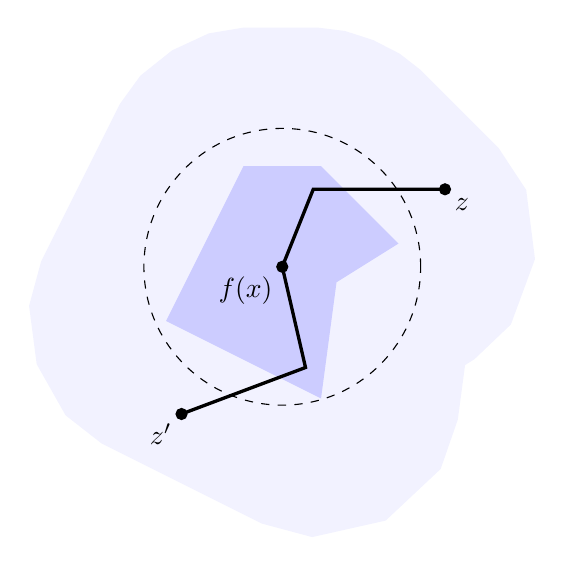
\begin{tikzpicture}[x=2.8em, y=2.8em]
    \draw[blue!05, line width = 10em, rounded corners] 
        (1,1) -- (3,0) -- (3.2,1.5) -- (4,2) -- (3,3) -- (2,3) -- (1,1) -- (3,0);
    \fill[fill=blue!20, very thick] 
        (1,1) -- (3,0) -- (3.2,1.5) -- (4,2) -- (3,3) -- (2,3) -- (1,1);
    \draw[very thick]
        (4.6,2.7) -- (2.9,2.7) -- (2.5,1.7) -- (2.8,0.4) -- (1.2,-0.2);
    \filldraw
        (2.5,1.7) circle(2pt) node[anchor=north east]{$f(x)$}
        (4.6,2.7) circle(2pt) node[anchor=north west]{$z$}
        (1.2,-.2) circle(2pt) node[anchor=north east]{$z'$};
    \draw[dashed]
        (2.5,1.7) circle(5em);
    \end{tikzpicture}
\end{center}
We have $K_x \subset B(f(x),\frac{\varepsilon}{5})\subseteq O_x := \frac{\varepsilon}{5}\text{-neighborhood of }K_x$. Hence both $z$ and $z'$ are at distance $\le\frac{\varepsilon}{5}$ from a point in $K_x$, and both these points are at distance $\le\frac{\varepsilon}{5}$ from $f(x)$. Thus, $d(z,z')\le4\frac{\varepsilon}{5}$.

As shown in the picture, for all $z,z'\in O_i$, we have $d(z,z')\leq 4\epsilon/5<\epsilon$ (to expand on this, observe we have $f(K_x) \subset B(f(x),\frac{\varepsilon}{5})\subseteq O_x := \frac{\varepsilon}{5}\text{-neighborhood of }f(K_x)$, hence both $z$ and $z'$ are at distance less or equal than $\frac{\varepsilon}{5}$ from two points of $f(K_x)$, and both these points are at distance less or equal than $\frac{\varepsilon}{5}$ from $f(x)$).

Suppose that $g\in W(K_1,O_1)\cap\dots\cap W(K_m,O_m)$. Then for all $x\in X$ there is $1\leq i\leq m$ with $x\in K_i$. Since $g\in W(K_i,O_i)$, we have $g(x)\in O_i$. We also have $x\in K_i=K_{x_i}$, so $d(f(x),f(x_i))\leq\epsilon/5$ so $f(x)\in O_i$. Hence $d(g(x),f(x))<\epsilon$. Since this holds for all $x\in X$, $d(f,g)<\epsilon$. So $W(K_1,O_1)\cap\dots\cap W(K_m,O_m)\subset B_{\sup}(f,\epsilon)\subset A$.
\end{proof}

% Lecture 10

\lecture[Legend has it that if you repeat compact-open for two hours loop spaces will appear.]{2021-11-17}

I missed this lecture, thanks to Paul for providing photos of the blackboard!

Up to now we have proved the following facts:
\begin{itemize}[label={-}]
    \item for a Hurewicz fibration (resp. Serre fibration) over a path-connected space, the fibres are homotopy equivalent (resp. the same, but whenever they admit CW-structures),
    \item fibre bundles, Hurewicz fibrations and Serre fibrations are stable under base change,
    \item if $X$ is compact and $Z$ is a metric space, the compact-open topology on $Z^X$ agrees with the topology of the supremum metric.
\end{itemize}

\begin{example}
Let $I$ be any set, endowed with the discrete topology. Let $Z$ be a space and consider $Z^I=\prod_I Z$. Then the compact-open topology on $Z^I$ agrees with the product topology.
\begin{itemize}
    \item Let $J$ be any subset of I; then $J$ is compact if and only if it is finite. So the sets $W(J,O)=\prod_{j\in J}O\times\prod_{j\not\in J}Z$ for $J$ finite and $O$ open form a subbasis of the compact-open topology. These sets are open in the product topology.
    \item A subbasis in the product topology is given by the sets $\prod_{j\in J}O_j\times\prod_{j\not\in J}Z$ for $J\subset I$ finite and $O_j$ open in $Z$. But then we have that
    \[\prod_{j\in J}O_j\times\prod_{j\not\in J}Z=\bigcap_{j\in J}(O_j\times\prod_{i\neq j}Z)=\bigcap_{j\in J}W(\cb{j},O_j)\]
    is open in the compact-open topology.
\end{itemize}
\end{example}

\begin{theorem}\label{theorem:compact-subbasis-topology}
Let $X$ and $Z$ be spaces and let $\S$ be a subbasis of the topology on $Z$. Then the sets $W(K,O)$ for $K\subset X$ compact and $O\in\S$ form a subbasis of the compact-open topology.
\end{theorem}

\begin{proof}
The "new topology" (generated by $W(K,O)$ for $O\in\S$) is clearly contained in the compact-open topology. We need to show that for all $O\subset Z$ open, the set $W(K,O)$ is in the new topology.

If $O\in\S$, this is true by definition.

If $O=\nns{O}{\cap}{n}$ with $O_i\in\S$, then
\[W(K,O)=W(K,O_1)\cap\cdots\cap W(K,O_n)\]
which is open in the new topology.

Now, suppose $O=\bigcup_{i\in I}O_i$ with $O_i\in\Bb$, where $\Bb$ is the basis generated by $\S$, i.e. the set of all finite intersections of sets in $\S$. Let $f\in W(K,O)$. Then for each $x\in X$ there is a set $O_x\in\Bb$ with $f(x)\in O_x\subset O$. Since $K$ is compact, hence locally compact, there is a compact neighbourhood $K_x$ of $x$ with $f(K_x)\subset O_x$. The covering $\cb{K_x}_{x\in K}$ of the compact set $K$ has a finite subcover $K\subset K_{x_1}\cup\cdots\cup K_{x_n}$. Then
\[f\in \bigcap_{i=1,\dots,n}W(K_{x_i},O_{x_i})\subset W(K,O).\]
\end{proof}

\begin{theorem}
Let $X$ and $Z$ be spaces and let $X$ be locally compact. Then the evaluation map $\ev:Z^X\times X\to Z,\ \ev(f,x)=f(x)$, is continuous.
\end{theorem}

\begin{proof}
Let $O$ be any open subset of $Z$. We want to show that
\[\ev^{-1}(O)=\cb{(f,x)\in Z^X\times X:f(x)\in O}\]
is open. Let $(f,x)\in Z^X\times X$ be in $\ev^{-1}(O)$, so $f(x)\in O$. Since $f$ is continuous, $f^{-1}(O)$ is an open neighbourhood of $x$. Since $X$ is locally compact, there is a compact neighbourhood $K$ of $x$ inside $f^{-1}(O)$. Then $f\in W(K,O)$ and $W(K,O)\times K$ is a neighbourhood of $(f,x)$ in $Z^X\times X$. Then $\ev(W(K,O)\times K)\subset O$, hence $(f,x)\in W(K,O)\times K\subset\ev^{-1}(O)$, so $\ev^{-1}$ is open.
\end{proof}

\begin{theorem}
Let $X,Y$ and $Z$ be spaces.
\begin{numerate}
    \setcounter{enumi}{-1}
    \item For every continuous map $f:X\times Y\to Z$, the adjoint map $\Phi(f):Y\to Z^X$, $\Phi(f)(y)(x)=f(x,y)$ is continuous. So $\Phi$ defines a map $Z^{X\times Y}\to(Z^X)^Y$.
    \item The map $\Phi:Z^{X\times Y}\to(Z^X)^Y$ is continuous.
    \item If $X$ is locally compact, then $\Phi$ is bijective.
    \item If $X$ is locally compact and $X$ and $Y$ are Hausdorff, then $\Phi$ is a homeomorphism.
\end{numerate}
\end{theorem}

\begin{proof}\ 

(0) Let $f:X\times Y\to Z$ be continuous and $\Phi(f):Y\to Z^X$ the adjoint map. To show that $\Phi(f)$ is continuous, it suffices to show that the sets $(\Phi(f))^{-1}(W(K,O))$ are open in $Y$ for all $K\in X$ compact, $O\in Z$ open. Let $y\in (\Phi(f))^{-1}(W(K,O))$, i.e. $f(K\times\cb{y})\subset O$, or $K\times\cb{y}\subset f^{-1}(O)$ which is open. By the tube lemma, there is a open neighbourhood $U$ of $y$ in $Y$ such that $K\times U\subset f^{-1}(O)$ or equivalently $\Phi(f)(U)\subset W(K,O)$. Hence $y\in U\subset(\Phi(f))^{-1}(W(K,O))$, so the latter set is open in $Y$.

(1) The compact-open topology on $Z^X$ has a subbasis consisting of the sets $W(K,O)$ for $K\subset X$ compact and $O\subset Z$ open. By theorem \ref{theorem:compact-subbasis-topology} the compact-open topology on $(Z^X)^Y$ has a subbasis of the form $W(K',W(K,O))$ for $K\subset X$ compact, $K'\subset Y$ compact, $O\subset Z$ open. But $\Phi^{-1}(W(K',W(K,O)))=W(K\times K',O)$ which is open in the compact-open topology on $Z^{X\times Y}$ because $K\times K'$ is again compact.

(2) On the set-theoretic level, every map $Y\to Z^X$ is of the form $\Phi(f)$ for some unique map $f:X\times Y\to Z$. So $\Phi$ is continuous by (1) and injective. We have to show that when $X$ is locally compact and $g:Y\to Z^X$ is continuous, $\Phi^{-1}(g)$ is continuous. But since the evaluation map is continuous by (0), the composite
\[\Psi(g):X\times Y\cong Y\times X\xto{g\times\id}Z^X\times X\xto{\ev}Z\]
is continuous, hence we have:
\[\Phi(\Psi(g))(y)(x)=\Psi(g)(x,y)=\ev(g(y),x)=g(y)(x)\text{ for all }x\in X,y\in Y\]
so that $\Phi(\Psi(g))=g$.

(3) Now we suppose that $X$ is locally compact Hausdorff and $Y$ is Hausdorff. As we saw in (1), the sets $W(K',W(K,O))$ with $K\subset X$ and $K'\subset Y$ compact, $O\subset Z$ open, form a subbasis on $(Z^X)^Y$. Then
\[\Phi^{-1}(W(K',W(K,O)))=W(K\times K',O)\]
so that we just need to show that the sets $W(K\times K',O)$ generate the compact-open topology on $Z^{X\times Y}$. This is the content of the following lemma.
\end{proof}

\begin{lemma}
Let $X$ and $Y$ be Hausdorff spaces and $Z$ any space. Then the compact-open topology on $Z^{X\times Y}$ is generated by the sets $W(K\times K',O)$ for all $K\subset X$ compact, $K'\subset Y$ compact and $O\subset Z$ open.
\end{lemma}

\begin{proof}
Let $L$ be any compact subset of $X\times Y$ and $O$ an open subset of $Z$. We need to show that $W(L,O)$ is open in the potentially small topology generated by the sets $W(K\times K',O)$. Let $f\in W(L,O)$ be arbitrary, we have $L\subset f^{-1}(O)$, which is open in $X\times Y$. For each $(x,y)\in L$ we can choose $U_{x,y}$ open in $X$ and $V_{x,y}$ open in $V$ with $(x,y)\in U_{x,y}\times V_{x,y}\subset f^{-1}(O)$. We set $L_X=\pr_X(L)$ and $L_Y=\pr_Y(L)$, which are quasi-compact subsets of $X$ and $Y$ respectively. Since $X$ and $Y$ are Hausdorff, $L_X$ and $L_Y$ are indeed compact, hence locally compact. For each $(x,y)\in L$ we can find compact neighbourhoods $K_{x,y}$ of $x$ in $L_X$ and $K'_{x,y}$ of $y$ in $L_Y$. Then the sets $\cb{K_{x,y}\times K'_{x,y}}_{(x,y)\in L}$ cover L. Since $L$ is compact, there is a finite subcover $\cb{K_{x,y}\times K'_{x,y}}_{(x,y)\in I}$ with $I$ finite. Then
\[f\in\underbrace{\bigcap_{(x,y)\in I}W(K_{x,y}\times K'_{x,y},O)}_{\text{open in the potentially smaller topology}}=W(\bigcup_{(x,y)\in I}K_{x,y}\times K'_{x,y},O)\subset W(L,O)\]
where the last inclusion follows from $L\subset \bigcup_{(x,y)\in I}K_{x,y}\times K'_{x,y}$.
\end{proof}

\begin{remark}
The assignment $(Z,X)\mapsto Z^X$ is a contravariant functor for continuous maps in Hausdorff spaces and a covariant functor for continuous map in all spaces, i.e.
\[(-)^{(-)}:\Top\times\Top^\op_{H}\to \Top\]

Contravariant functoriality: let $f:X\to X'$ be a continuous map between Hausdorff spaces. Define $f^*:Z^{X'}\to Z^X$ by precomposition with $f$, i.e.
\[f^*(\psi:X'\to Z)=\psi\circ f:X\to Z.\]

This map is continuous: let $K\subset X$ be compact, $O\subset Z$ open, then
\[(f^*)^{-1}(W(K,O))=\cb{\psi:X'\to Z\mid (\psi\circ f)(K)\subset O}=W(f(K),O).\]
Since $K$ is compact, $f(K)$ is quasi-compact; since $X'$ is Hausdorff, $f(K)$ is compact.

Covariant functoriality: let $g:Z\to Z'$ be continuous. We define $g_*:Z^X\to (Z')^X$ by postcomposition with $g$, i.e.
\[g_*(\psi:X\to Z)=g\circ\psi:X\to Z'.\]

This map is continuous: let $K\subset X$ be compact and $O\subset Z'$ open, then
\[g_*^{-1}(W(K,O))=\cb{\psi:X\to Z\mid (g\circ\psi)(K)\subset O}=W(K,g^{-1}(O))\]
which is open in $Z^X$.

Note also that for $f:X\to X'$ continous, $g:Z\to Z'$ continuous and $X,X'$ Hausdorff, the following square commutes:
\begin{center}
    \begin{tikzcd}
    (Z')^{X'} \arrow[r,"f^*"] & (Z')^X\\
    Z^{X'} \arrow[u,"g_*"] \arrow[r,"f^*"] & Z^X \arrow[u,"g_*"]
    \end{tikzcd}
\end{center}
\end{remark}

\begin{example}
Let $f,g:X\to Z$ be homotopic maps, with $H:X\times[0,1]\to Z$ a homotopy between them. The adjoint $\Phi(H):[0,1]\to Z^X$ is then continuous. Hence homotopies correspond to paths in $Z^X$, so that the map:
\begin{align*}
[X,Z]&\to\pi_0(Z^X)\\
[f]\ \ &\mapsto\ \ [f]
\end{align*}
where $[X,Z]$ indicates the set of homotopy classes of maps $X\to Z$, is well-defined and a bijection whenever $X$ is locally compact.
\end{example}

\section{Path Spaces and Loop Spaces}

For a space $X$, the space $X^{[0,1]}$ is the \textbf{path space} of $X$. For a pointed space $(X,x_0)$, the \textbf{loop space} $\Omega X$ is the subspace of $X^{[0,1]}$ consisting of all loops at $x_0$, i.e. those $\omega\in X^{[0,1]}$ with $\omega(0)=\omega(1)=x_0$.

Let $q:[0,1]\to S^1=\cb{z\in\CC\mid|z|=1}$ be the quotient map $q(x)=e^{2\pi ix}$, this induces a continuous map
\[q^*:X^{S^1}\to X^{[0,1]},\]
which restricts to a continuous bijection onto $\Omega X$
\[(X,x_0)^{(S^1,1)}=\cb{f:S^1\to X\mid f(1)=x_0}.\]
This is in fact a homeomorphism, as a special case of the following lemma.

\begin{lemma**}
Let $q:X\to Y$ be a quotient map between compact spaces. Then for every space $Z$, the continuous map $q^*:Z^Y\to Z^X$ is a homeomorphism onto the subspace of all functions $f:X\to Y$ that factor through $q$.
\end{lemma**}


%%% Appendix

\chapter{Appendix}

\section{Interesting exercises}

\begin{exercise!}[Homology and homotopy groups of telescope]
Write it!\todo{add text}
\end{exercise!}

\begin{solution}
Do it!\todo{add solution}
\end{solution}

\section{Things to see}



\nocite{*}


\backmatter\KOMAoption{chapterprefix}{false}
\printbibliography[heading=bibintoc, title={References}]
\end{document}
